\documentclass[a4paper,10pt]{article}
\usepackage[utf8]{inputenc}
\usepackage{courier}
\setcounter{tocdepth}{2} %Only show sections and subsections in toc.

\usepackage{longtable} %used for acro
\usepackage{acro} %list of acronyms

%!TEX root = ../main.tex
\DeclareAcronym{ui}
{
	short = {UI},
	long = {User Interface}
}

\DeclareAcronym{gui}
{
	short = {GUI},
	long = {Graphical User Interface}
}

\DeclareAcronym{gps}
{
	short = {GPS},
	long = {Global Positioning System}
}

\DeclareAcronym{zybo}
{
	short = {ZB},
	long = {Zybo Board}
}

\DeclareAcronym{can}
{
	short = {CAN},
	long = {Controller Area Network}
}

\DeclareAcronym{pdo}
{
	short = {PDO},
	long = {Process Data Object}
}

\DeclareAcronym{sdo}
{
	short = {SDO},
	long = {Service Data Object}
}

\DeclareAcronym{cep}
{
	short = {CEP}
	long = {Circular Error Probability}
}


\usepackage{colortbl}
\usepackage{siunitx} %Package for SI units
\sisetup{per-mode=fraction}
\usepackage{mathdots}
\usepackage{textcomp} %Vertically centered tilde (~)
\usepackage{amsmath}
\usepackage{graphicx,booktabs}
\usepackage{standalone}
\usepackage{rotating,booktabs}
\usepackage{lscape} % to rotate OD table
\usepackage{array,etoolbox}
\preto\tabular{\setcounter{magicrownumbers}{0}}
\newcounter{magicrownumbers}
\newcommand\rownumber{\stepcounter{magicrownumbers}\arabic{magicrownumbers}}

\usepackage[font={footnotesize}]{caption}
\usepackage[font={footnotesize}]{subcaption}

\newcommand{\mikkel}[1]{\todo[inline,linecolor=green!100,backgroundcolor=red!70, bordercolor=green, author = Mikkel]{#1}}
\newcommand{\martin}[1]{\todo[inline,color=blue!30, author = Martin]{#1}}
\newcommand{\thomas}[1]{\todo[inline,color=black!30, author = Thomas]{#1}}
\newcommand{\catalin}[1]{\todo[inline,color=green!100, author = CataLinux]{#1}}
%newcommand{\bb}[1]{\mathbb{#1}}

%\usepackage{hyperref}

%\hypersetup{
%    colorlinks = false,
%    linkbordercolor = {white},
%}


%\hypersetup{
 %   colorlinks,
 %   linkcolor={red!50!black},
 %   citecolor={blue!50!black},
 %   urlcolor={blue!80!black}
%}

\usepackage{float}
\usepackage[procnames]{listings}
\usepackage{epstopdf} %Convert EPS files to PDF format
\usepackage{pdfpages} %Utility to include pdf documents into the report, used to include datasheets in appendices.

\usepackage{tikz} 			%Utility to draw nice figures
\usetikzlibrary{shapes.geometric, arrows}
\usepackage{standalone}
\usepackage{circuitikz} 	%Utility to draw circuits in tikz

\usepackage[T1]{fontenc}	% Quotes
\usepackage{dblfloatfix}	% used to have a headline on a page with a rotated table
\usepackage{todonotes}
\usepackage{listings}
\lstset{
backgroundcolor = \color{black!5},
tabsize=3,
frame=l,
language=c++,
escapeinside={(*@}{@*)},
basicstyle=\small\ttfamily,,
numbers=left,
numberstyle=\tiny\color{gray},
keywordstyle=\color{blue},
commentstyle=\color{green}\ttfamily,
stringstyle=\color{gray},
upquote=true,
breaklines = true
  }
\renewcommand{\lstlistingname}{Code} %Let listings have code instead of figure
\usepackage{tabularx}

\usepackage{multirow}

\usepackage{url}
\renewcommand{\UrlFont}{\large\tt}

\usepackage{chngcntr} %Change the counters of objects. Used to make figure/table and equation counting specific to the section they are in.
\counterwithin{figure}{section}
\counterwithin{equation}{section}

\setcounter{tocdepth}{2}

%Make counter of listings specific to sections
\AtBeginDocument{%
\counterwithin*{lstlisting}{section}
  \renewcommand{\thelstlisting}{%
  \ifnum\value{subsection}=0
      \thesection.\arabic{lstlisting}%
      \else
      \ifnum\value{subsubsection}=0
        \thesection.\arabic{lstlisting}%
        \else
        \thesection.\arabic{lstlisting}%
        \fi
        \fi
  }%
  }

%\usepackage[inner=2cm,outer=4cm]{geometry}

\setlength{\parindent}{0pt}

\title{Electronics - 2. Semester Project}
\author{Thomas Søndergaard Christensen, Mikkel 
Skarup Jaedicke, Martin Brøchner Andersen, Catalin Ionut Ntemkas‎}
\date{dd/mm/2016}

\begin{document}
%!TEX root = ../main.tex
\begin{titlepage}
%\newgeometry{left=3cm,right=3cm}
\begin{center}

\textsc{\LARGE University of Southern Denmark}\\[1.5cm]
\textsc{\Large MSc in Engineering - Electronics}\\
\textsc{\large 2. Semester Project}\\[0.5cm]

\vfill
\vspace{3cm}
\hrule ~\\[0.3cm]
{ \LARGE \bfseries We need a title\\[0.4cm] }
\hrule ~\\[1.5cm]

\vfill

%\includegraphics[width=0.3\textwidth]{graphics/sdu_logo}
\vspace{7cm}
% Author and supervisor
\begin{minipage}[t]{.49\textwidth}
\begin{flushleft} \large
\textbf{Authors:}\\
230390 Martin Brøchner Andersen\\
430583 Catalin Ionut Ntemkas\\
030192 Mikkel Skaarup Jaedicke\\
100589 Thomas S. Christensen
\end{flushleft}
\end{minipage}
\begin{minipage}[t]{.49\textwidth}
\begin{flushright} \large
\textbf{Supervisors:} \\
Leon xxxxx
\end{flushright}
\end{minipage}

\vspace{1cm}
Date: xx-xx-2016

\vspace{1cm}

\end{center}
%\restoregeometry
\end{titlepage}
\newpage
\pagenumbering{Roman}
%!TEX root = ../main.tex
\section*{Preface}
\addcontentsline{toc}{section}{Preface}

\section*{Acknowledgment}
\addcontentsline{toc}{section}{Acknowledgment}
This project would not have been possible without the invaluable assistance and patience of our supervisor. 
A Tremendous thank you to Leon Bonde Larsen.
The process was simplified by Assistant Professor Kjeld Jensen from which the sensory equipment used in the report was supplied.
\thomas{Rewritten - needs a bit more?}
\martin{Who else should we thank? Viking Pizza?}
\mikkel{NEW URL}
\vspace{5cm}
\begin{center}
	\begin{minipage}[t]{.55\textwidth}\large
		\begin{center}
		Catalin Ionut Ntemkas\\
		\vspace{1cm}
		\hrule
		\vspace{0.5cm}
		Martin Brøchner Andersen\\
		\vspace{1cm}
		\hrule
		\vspace{0.5cm}
		Mikkel Skaarup Jaedicke\\
		\vspace{1cm}
		\hrule
		\vspace{0.5cm}
		Thomas Søndergaard Christensen
		\vspace{1cm}
		\hrule
		\end{center} 
	\end{minipage}
\end{center}

\vspace{1.2cm}
  \begin{center}
    \textsl{The report, source code, data, plotting script and simulations can be found at:}  
    \end{center}
    \vspace{-5pt}
    \begin{center}
	\renewcommand{\UrlFont}{\color{black}\normalsize\tt}
    \url{github.com/mikkeljae/SEM1PRO_ELECTRONICS}
   \end{center}
\newpage

\section*{Abstract}
\addcontentsline{toc}{section}{Abstract}
A go-kart has been supplied as a development platform for student projects at University of Southern Denmark.
In the interest of enabling more complex projects, a unified data collection system is necessary.
This is developed throughout this report. 
An analysis is done to determine the requirements of such a system.
It was found that a two-part network is suitable for this application.
The two parts are a CAN network and an ad-hoc WiFi network.
A custom protocol for use on CAN, GoCAN, is developed.
GoCAN supports up to 16 sensors from which data can be monitored on a remote monitoring station using the WiFi connection.
The system was only partially implemented since a connection between the CAN network and Linux was not achieved.
\thomas{Rewritten}
\newpage
\tableofcontents
\newpage
\listoftodos
\listoffigures
\listoftables
\addcontentsline{toc}{section}{Acronyms}
\printacronyms
\clearpage
\newpage
\pagenumbering{arabic}
\part{Preface}
%!TEX root = ../main.tex
\section{Introduction} % (fold)
\label{sec:introduction}
Something here....
\catalin{yearh!}
% section introduction (end)
\newpage
%!TEX root = ../main.tex
\section{Monitoring of sensor data on the SDU go-kart.}
This project aims to produce a tool for developing, evaluating and testing hardware for the SDU go-kart.
Movement of the go-kart should be monitored to enable evaluation of the performance of the go-kart.
The control variables and currents of the inverter should be monitored in order to help develop new hardware or evaluate existing hardware.
A basic use case diagram showing the functionality of the system can be seen in figure \ref{fig:use_cases}.
The use case narratives are shown in tables \ref{tab:use_monitor} to \ref{tab:use_read_log}.
\begin{figure}[h]
 	\centering
    \includegraphics[width=0.8\textwidth]{graphics/use_cases}
    \caption{Use case diagram for the system.}
    \label{fig:use_cases}
\end{figure}


\begin{table}[]
\centering
\caption{Usecase narrative for monitor live data from go-kart.}
\label{tab:use_monitor}
\begin{tabular}{| r | p{6 cm} |}
\hline
\textbf{Use case:}                        & Monitor live data from go-kart                  \\ 
\textbf{Actors:}                          & Engineer                                        \\
\textbf{Purpose:}                         & Monitor live data from go-kart                  \\
\textbf{Overview:}                        & The engineer starts the system. The system will begin collecting data on the go-kart and transfer them to a stationary computer. The computer will present data to the engineer on a GUI. \\
\textbf{Type:}                            & Essential                                       \\
\textbf{Preconditions:}                   & -                                               \\
\textbf{Postconditions:}                  & System transfers data from go-kart sensors to a stationary computer, showing data in a GUI.                                                                                            \\
\textbf{Special requirements:}            & -                                               \\ \hline 
\multicolumn{1}{|c|}{\textbf{Actor action}} & \multicolumn{1}{c|}{\textbf{System response}}\\
\multicolumn{1}{|l|}{1. Start system}       & \begin{tabular}[c]{@{}l@{}}2. Start collecting data\\ 3. Transfer data to stationary computer\\ 4. Present data in GUI\end{tabular}                                              \\ \hline
\multicolumn{2}{|c|}{\textbf{Alternative flow of events}}                                   \\
\multicolumn{2}{|p{12 cm}|}{Any line: User can stop the system at any point in time.}              \\ \hline                                                                                                                                    
\end{tabular}
\end{table}


\begin{table}[]
\centering
\caption{Usecase narrative for log go-kart data.}
\label{tab:use_log}
\begin{tabular}{| r | p{6 cm} |}
\hline
\textbf{Use case:}                        & Log go-kart data            			        \\ 
\textbf{Actors:}                          & Engineer                                        \\
\textbf{Purpose:}                         & Log go-kart data                 				\\
\textbf{Overview:}                        & After startup the system will log the collected go-kart data on xx  \\
\textbf{Type:}                            & Essential                                       \\
\textbf{Preconditions:}                   & System is running and collecting go-kart data   \\
\textbf{Postconditions:}                  & System logs collected go-kart data.      		\\
\textbf{Special requirements:}            & -                                               \\ \hline 
\multicolumn{1}{|c|}{\textbf{Actor action}} & \multicolumn{1}{c|}{\textbf{System response}} \\
\multicolumn{1}{|l|}{}       & \begin{tabular}[c]{@{}l@{}}1. Log collected data\end{tabular}\\ \hline
\multicolumn{2}{|c|}{\textbf{Alternative flow of events}}                                   \\
\multicolumn{2}{|p{12 cm}|}{Any line: User can stop the logging	 at any point in time.}         \\ \hline                                                                                                                                    
\end{tabular}
\end{table}



\begin{table}[]
\centering
\caption{Usecase narrative for read logged data.}
\label{tab:use_read_log}
\begin{tabular}{| r | p{6 cm} |}
\hline
\textbf{Use case:}                        & Read logged data  			                    \\ 
\textbf{Actors:}                          & Engineer                                        \\
\textbf{Purpose:}                         & Monitor live data from go-kart                  \\
\textbf{Overview:}                        & The engineer will ask the system for the logged data. The system will transfer the logged data to a stationary computer \\
\textbf{Type:}                            & Essential                                       \\
\textbf{Preconditions:}                   & Data is logged in logfile on xx                 \\
\textbf{Postconditions:}                  & The log file is on the stationary computer                                                                                      \\
\textbf{Special requirements:}            & -                                               \\ \hline 
\multicolumn{1}{|c|}{\textbf{Actor action}} & \multicolumn{1}{c|}{\textbf{System response}}\\
\multicolumn{1}{|l|}{1. Ask for log file}       & \begin{tabular}[c]{@{}l@{}}2. Transfer logged data to statinary computer\\ 3. Save data to log file on stationary computer\end{tabular}                                              \\ \hline
\multicolumn{2}{|c|}{\textbf{Alternative flow of events}}                                   \\
\multicolumn{2}{|p{12 cm}|}{Any line: If connection is lost the system should detect it and mark the trasferred log file as invalid}              \\ \hline                                                                                                                                    
\end{tabular}
\end{table}



%Relavant control variables should be controllable, while driving allowing for efficient testing of controllers.
To achieve this, data should be collected on a computer on the go-kart and sent to a stationary computer.

%\subsection{What is the role of transferring go-kart data to and from a stationary computer?}
%To let an engineer or a mechanic monitor the status of the go-kart.

%Movement data could be usefull for testing new hardware, improving existing hardware and evaluation the drivers performance. 
%Data about battery status, currents, motortemperature is usefull for safety procedures.
%Data from the SEVCON xxx inverter or other inverters on the go-kart could be used for tuning parameters, evaluation performance and safety measures.
%On the basis of this data it should be possibly to change configuration parameters on the SEVCON xxx while driving the go-kart.

\subsection{What is the role of the stationary computer?}
The stationary computer should be responsible of the transmission of relevant go-kart data to and from the "on-board" computer.
The received data should be presented to the user in a SCADA system.

\subsubsection*{What data and sensors would be interesting to monitor?}
Data from IMU, GPS and encoders would be necessary to monitor the movement of the go-kart.
Data from the SEVCON xxx gives information about about battery status, currents, motortemperature.
%Temperature of tyres, speed of front wheels, possibility to control or at least moniter stearing and brake.
It should be possible to get data from a new inverter, that is not yet made. 

\subsubsection*{What kind is the stationary computer?}
It should be possible for different personnel to monitor the go-kart data therefore the statinonary computer should just be general purpose computer running (linux?).

\subsubsection*{What kind of communication is needed to transfer data between the go-kart computer and the stationary computer?}
As it should be possibly to monitor data while the go-kart is driving the connection clearly needs to be wireless with a range allowing for driving on a typical racing track. 
As all data is used by humans the propagation delay of the connection is not required to be very low.

\subsubsection*{How should data on the stationary computer be presented?}
As live data should be easy to read? ("overskue" in danish) there needs to be a GUI or at least a UI that will present the user with easy readable data. SCADA SYSTEM!?!?!
Changing of parameters on the go-kart should also be in the UI in order useable by others than the developers.

\subsection{What is the role of the computer on the go-kart?}
The "onboard" computer needs to handle the collection
of data from different sensors (data producers).
This computer will also handle the transmission of data to the stationary 
computer.
%There are tasks that need to be handled locally fx strict safety measures (and future things fx localisation) that requires a miminum delay. 
Storing of data with a 
The computer needs also to store data locally in order to avoid data loss if the wireless connection is lost.

\subsubsection*{How is local data transmission handled?}
All data should be collected locally on the "on-board" computer to transmit it to the stationary computer.
Local data collection should be "fast" and "reliable" for local safety measures to function properly.
It should be possibly to collect data from and transmit data to at least the 
aforementioned IMU, GPS and SEVCON xx with the possibility of adding additional 
data producers.

\subsubsection*{What kind is the "on-board" computer?}
The computer should be a small embedded platform in order to mount it physcically on the go-kart.
It should be able to handle all "on-board" tasks.

\subsubsection*{How should local data storage be realised?}
Data should be stored directly on nonvolatile memory to be able retrieve data after shutdown.
Data integrity checks is needed to ensure proper data logging.
%Correct data logging should be realised to ensure validity of data. 


\newpage
\section{System requirements}

\subsection{Actors}
The only actor on the system is an engineer.

\subsection{Interfaces}
\begin{itemize}
\item Wifi, for data transfer between go-kart and stationary computer.
\item CAN bus, for local network.
\item CanOpen, for interfacing the Sevcon.
\item USB, for GPS and IMU.
\item ??, for SD card connection.
\item Powersupply, for Zybo boards.
\end{itemize}

\subsection{Functional requirements}
The system: 
\begin{itemize}
\item Reads data from sensors.
\item Reads data from Sevcon.
\item Transfers data to stationary computer using Wifi.
\item Presents data to the user.
\item Logs sensordata to SD card.
\item Read data from SD card.
\item Timestamps all data. 
\end{itemize}

\subsection{Operational requirements}
The system monitors go-kart data.% when engineer starts the system by powering it on.

\subsection{Quality of service requirements}
\begin{itemize}
\item IMU data must be sampled with xx Hz.
\item GPS data must be sampled with zz Hz.
\item Data logging with qq Hz.??
\end{itemize}

\subsection{Parametric requirements}
Wifi range must be greater than xx meters.

\subsection{Design requirements}
The system:
\begin{itemize}
\item must be scalable to at least 16 sensors/nodes.
\item must be modular to allow easy integration of new sensors/nodes.
\item must be functional if one or more sensors/nodes stop working.	 
\end{itemize}



\newpage
\section{Further ivestigation}

\subsection{Parameters of Interest}
\label{sec:parameters}
In developing new hardware or evaluating current hardware, it is necessary to be able to monitor a range of parameters.
This section will investigate what parameters need to be logged in order to provide a useful and complete logging of the behaviour of the go-kart.
The parameters in question fall into three categories; Physical parameters, electrical parameters and mechanical parameters.
These will be dealt with in turn in the following sections
\paragraph*{Physical Parameters}
This category comprises all information about the motion of the go-kart.
\begin{itemize}
	\item \textbf{Position, Absolute:} Providing a means to record the absolute position of the go-kart is a useful feature in certain fields.
	Especially any form of localisation and pathfinding will be able to put this information to use.
	The absolute position of the go-kart can be recorded using a GPS module or possibly by using a known starting coordinate and information about the relative movement of the go-kart.
	\item \textbf{Position, Relative:} The relative position of the kart can be, as just mentioned, used to infer the absolute position of the go-kart.
	Additionally it can provide a means to analyze a drivers performance on the track or detect drift while cornoring.
	The relative position includes both translational, as well as rotational information.
	This information can be gathered using an inertial measurement unit (IMU).
	An IMU is a compound device, comprising of an accelerometer and a gyroscope and, in some cases, a magnetometer.
	\item \textbf{Velocity:} The velocity of the go-kart is key in optimising lap-times, clearly, it is desirable to monitor this parameter.
	It can be extracted by reading the motor encoders.
	However, the driving wheels are prone to slippage when cornoring, this would give an inaccurate reading of the actual velocity of the go-kart.
	Instead, a simple encoder can be mounted on either one, or both of the front wheels as these are freerunning and independent.
	Once the rotational speed of the axle is known, the velocity of the go-kart can be infered using the tyre diameter.
	\item \textbf{Acceleration:} It may be of interest to monitor the forces exerted on the go-kart, or, its acceleration, as it drives on the track.
	This information is already provided by the accelerometer in the IMU mentioned above and as such provides no additional complication.
\end{itemize}
Three sensors are mentioned in this section.
A GPS, an IMU and an encoder.
In order to limit the scope of the project only the GPS and the IMU will be implemented.
\paragraph*{Electrical Parameters}
This category comprises all information about the electrical aspects of the go-kart.
\begin{itemize}
	\item \textbf{Motor Currents:} Providing a means of monitoring the currents flowing through the motor allows the user to calculate the torque exerted by the motor as well as the current power draw of the motor.
	Knowing the currents could also prove an invaluable debugging tool when developing a new inverter for the go-kart.
	\item \textbf{Throttle Position:} The throttle on the go-kart is connected to a potentiometer.
	Measuring the voltage output of this potentiometer provides a simple way of monitoring the position of the throttle.
	\item \textbf{Desired Currents:} Based on the current throttle position a set of desired currents are calculated.
	Monitoring these allows spotting any discrepancies between the desired and the actual currents.
	\item \textbf{Duty Cycles:}
	\item \textbf{Battery Voltage:} As the go-kart is electrical, naturally, it has a battery.
	Monitoring the current battery status could give the user an indication of how much driving time is left, or how long until the batteries are recharged afterwards.
	\item \textbf{Motor Angle:} Knowing the angle of the motor at all times gives a means of more accurately calculate the currents at specific times.
	Additionally, it can be used in Clarke-Parke transformations, again, providing information in debugging an inverter in development.
\end{itemize}
These parameters are all available from the sevcon gen4 motor controller mounted on the go-kart.
This controller has a CANopen interface from which this data can be extracted.
Any users who wish to add their own inverter will simply need to obey the API stated by the sevcon gen4 CANopen interface in order to correctly log the data.
\paragraph*{Mechanical Information}
This category comprises all information about the mechanical aspects of the go-kart.
\begin{itemize}
	\item \textbf{Steering Wheel Angle:} Monitoring the angle of the steering wheel allows analysing the performance of the driver.
	In addition it opens up for the possibility of mechanical control of the go-kart.
	Similarly to monitoring the velocity, the steering wheel angle can be monitored by adding an encoder to the steering column.
	\item \textbf{Braking Pedal Position:} The braking system on the go-kart is similar to that of an ordinary car.
	The braking disc is mounted on the driving axle and the braking calibers connected to the brake pedal by a series of oil-filled hoses.
	Monitoring its actuation allows analysing the performance of the driver and as mentioned above, may potentially allow for mechanical control of the go-kart
\end{itemize}
As both of these parameters would require mechanical changes to the go-kart, they are beyond the scope of this project and as such will not be implemented.
\subsubsection*{Conclusion}
In this section a multitude of different parameters have been discussed.
Most of them can be logged using just three components; a Sevcon Gen4 motor controller, an IMU and a GPS.
These are the three components from which data logging will be implemented throughout this project.
This provides a solid platform to prove the concept and additional sensory equipment can be added at a later date, should it be required.

\subsection{Hardware for Monitoring Parameters}
In section \ref{sec:parameter} an overview of the different parameters that may be of interest for logging is given.
It was concluded that three components would suffice as a proof of concept; the Sevcon Gen4 motor controller, an IMU and a GPS.
This section will explore in more detail what requirements and communication schemes exists for each of the components.

\subsubsection*{Sevcon Gen4 Motor Controller}

\subsubsection*{Inertial Measurement Unit (IMU)}
IMU's, generally, exist in two versions.
A 6D and a 9D version.
Both include an accelerometer and a gyroscope.
In addition to these the 9D IMU includes a magnetometer, enabling measurement of absolute direction, as opposed to the relative measurement of direction granted by the magnetometer.
The requirement in terms of each of these parts is given as:
\begin{itemize}
	\item \textbf{Accelerometer [\si{\metre\per\second^2}]:} As the name implies, the accelerometer measures accelerations.
	That is, when the component changes speed or direction the force exerted on the accelerometer is measured.
	Professional drivers using professional grade go karts driving upwards of 250 \si{\kilo\metre\per\hour} can reach up to 2-3 g's of force exerted on them.
	The go kart available in this project has a theoretical maximum speed of 50 \si{\kilo\metre\per\hour}.
	Clearly, the forces exerted on this platform will be lower, however, a minimum requirement of $\pm$ 3g will be set for the accelerometer in the IMU.
	\item \textbf{Gyroscope [\si{\degree\per\second}]:} 
\end{itemize}
\subsubsection*{Global Positioning System (GPS)}
%\subsubsection{What is the data on stationary computer intended for?}
%Monitoring data related to movement from the go-kart and adjusting go-kart control parameters by an engineer.

%\subsubsection{What kind of data}
%Data from Sevcon controller related to the motor (control, temperature, speed etc.), and from other nodes that are sensors. Sensors may include IMU, GPS... (to be discussed).

%\subsubsection{What is meant by "computer"}
%Stationary computer is a laptop/desktop (general purpose computer, OS: Windows/Linux), and the go-kart computer is a zybo board running Linux.

%\subsubsection{What setup should be used for communication (Wireless/wired), what protocol etc.}
%Wireless communication to make possible the monitoring/adjusting while the go-kart is being driven on a track. Protocol?

%\subsubsection{Does the communication require extra verification? checksum, timestamping etc.?}
%YES.


%\subsubsection{How many nodes/sensors should the system be able to handle?}
%The system will be scalable. How much will be discussed.

%\subsubsection{What kind of nodes/sensors/actuators?}
%Sevcon and possibly IMU, GPS...

% \subsubsection{QUESTIONS - should be deleted. They are only here for inspiration.}
% \begin{itemize}{}
% \item What bandwidth/latency should the communication be able to handle?
% \item How is data produced? i.e. just by the sensors, by the go-kart or both systems?
% \item How many sensors/data producers?\\
% \item Should we support asynchronous transfer? (different sensors with different 
% update frequency transfer at different rates).\\
% \item Which tasks should be handled where? i.e. can some tasks be handled locally on 
% the go-kart?
% \item What topology should the go-kart network be? Ring?
% \item What should the basic gui (on the laptop) be?
% \item Go-kart network hierarchy? A zybo master ruling the rest puny zybos without mercy?
% \item Required hardware to make the entire network? (eg. Zybos, pmod ip core ethernet, wifi card for zybo etc.)
% \item Sevcon requires use of OpenCan. How will the connection between the Sevcon and the network should be done?
% \item What is the max distance we want to support for wireless communication Stat. Laptop - Go-kart zybo? What hardware for that distance?
% \item How does this max distance affects the bandwidth/latency and in general, the efficiency of the entire network?
% \item If we have error-handling on the go-kart zybo, what kind of errors might those be?!??!
% \item Programming language/IDE of creating the GUI?
% \item How the failure of a node will be handled?
% \item How the wifi disconnection between Stationary PTP-LINKC and the go-kart zybo will be handled? A msg in GUI? What about if data was being transmitted, should we check if the node got the data? In other words, do we need verification of data received by the nodes shown on the gui after adjusting the parameters?
% \item Embedded linux on one or all the nodes?

% \end{itemize}

\subsection{Wireless transmission}
The wireless transmission between the go-kart computer and the stationary computer could be a number of different technologies.
This section seeks to find an appropriate one.

\subsubsection{Range}
The range of the transmission is determined by the length of the test track. 
Normally the SDU kart is tested on parking lots with a maximum lenght of 50m and width of 20m.
There are almost no obstacles for the transmission on such a parking lot. 
This test track sets a minimum requirement that the wireless setup should be able to transmit data at 55m with no obstacles.
\\
At some point it would be interesting to test the go-kart on a real go-kart track. 
The nearest go-kart track is \textit{Odense gokart Hal}, which is also thought to be an average indoor go-kart track.
The track is about 70m long and 40m in width with no obstacles other than the barriers. 
If the wireless transmitter and receiver are placed above the barrier then they will not an obstruction on the transmission. 
This track sets a minimum requirement of 80m transmission. 

\subsubsection{Speed}
The transferred data is from xx sensors producing a maximum of yy bites per sample. 
Data is only used for human inspection and therefore a sample frequency of 100Hz would be sufficient.
This gives a minimum requirement for the speed of the transmission to be ZZ Mbit/s. 

\subsubsection{Compatibility}
It should be possibly to change the stationary computer and therefore the chosen wireless transmission technology should be compatible with standard computers running linux.
The chosen hardware should be compatible with standard linux computers and the Zybo board. 
Both have USB ports and Ethernet ports as a standard, therefore the chosen hardware should one of those.

\subsubsection{Technologies}
Bluetooth is a technology that is compatible with standard computers running linux. 
Bluetooth 5.0 has a maximum speed of 50Mbit/s, which is sufficient.
The range of typical class 2 Bluetooth device is 10m \footnote{https://en.wikipedia.org/wiki/Bluetooth}.
This range is definitely not enough for this application.
\\
\\  
WiFi is also compatible with standard computers running linux and typical WiFi units has speeds that is a lot higher than the required. 
WiFi can be operating in the 2.4GHz band and in the 5GHz band. 
2.4GHz units has the highest range. 
The 802.11n protocol generally has the best range compared to the other 802.11 protocols \footnote{https://en.wikipedia.org/wiki/IEEE\_802.11\#802.11n}.
\\
A local network between computers without connection to existing networks such as the internet is referred to as an ad-hoc network. 
It is a required that the found hardware is capable of doing an ad-hoc network.

\subsubsection{Conclusion} 

\begin{table}[]
\centering
\caption{Minimum requirements for wireless transmission.}
\label{tab:req_wifi}
\begin{tabular}{|l|}
\hline
80m transmission             \\ \hline
ZZ Mbit/s                    \\ \hline
802.11n protocol             \\ \hline
USB or Ethernet              \\ \hline
ad-hoc network compatability \\ \hline
\end{tabular}
\end{table}
Based on the requirements in table \ref{tab:req_wifi} it was chosen to us the TP-LINK TL-WN722N, as it uses the 2.4GHz band, the 802.11n protocol, is compatible with linux, has an external antenna and uses USB. 

\newpage
\part{Analysis}
%!TEX root = ../main.tex
\section{System Analysis} % (fold)
\label{sec:system_analysis}
A thorough system analysis is needed in order to design an embedded system that meets the needs expressed by the use cases. 
This section will present the analysis of the complete embedded system, through the following topics:

\begin{itemize}
\item Parameters of interest. The use cases do not describe what parameters should be monitored meaning that it should be investigated which are relevant to monitor.
\item Hardware for monitoring parameters. It should be analysed what hardware is necessary in order to measure the parameters found to be relevant. 
\item Amount and frequency of data????. Something clever about this. Martins sections should be used for it.
\item Data collection. It should be analysed how data is collected on the go-kart.
\item Micro-controller. It should be analysed what micro-controller should be used on the go-kart.
\item Wireless network. It should be analysed how data is transferred from the go-kart 	to the stationary computer.
\item Local storage. There needs to local storage on the go-kart and it needs to be analysed what kind this should be and how it should be implemented.
\item Software on stationary computer. It should be be analysed how the software on stationary should prensent the transferred data to the user in an UI.
\end{itemize}

\subsection{Parameters of Interest}
\label{sec:parameters}
In developing new hardware or evaluating current hardware, it is necessary to be able to monitor a range of parameters.
This section will investigate what parameters need to be logged in order to provide a useful and complete logging of the behavior of the go-kart.
The parameters in question fall into three categories; Physical parameters, electrical parameters and mechanical parameters.
These will be dealt with in turn in the following sections
\paragraph*{Physical Parameters}
This category comprises all information about the motion of the go-kart.
\begin{itemize}
	\item \textbf{Position, Absolute:} Providing a means to record the absolute position of the go-kart is a useful feature in certain fields.
	Especially any form of localisation and path finding will be able to put this information to use.
	The absolute position of the go-kart can be recorded using a GPS module or possibly by using a known starting coordinate and information about the relative movement of the go-kart.
	\item \textbf{Position, Relative:} The relative position of the kart can be, as just mentioned, used to infer the absolute position of the go-kart.
	Additionally it can provide a means to analyze a drivers performance on track the or detect drift while cornoring.
	The relative position includes both translational, as well as rotational information.
	This information can be gathered using an inertial measurement unit (IMU).
	An IMU is a compound device, comprising of an accelerometer and a gyroscope and, in some cases, a magnetometer.
	\item \textbf{Velocity:} The velocity of the go-kart is key in optimising lap-times, clearly, it is desirable to monitor this parameter.
	It can be extracted by reading the motor encoders.
	However, the driving wheels are prone to slippage when cornoring, this would give an inaccurate reading of the actual velocity of the go-kart.
	Instead, a simple encoder can be mounted on either one, or both of the front wheels as these are freerunning and independent.
	Once the rotational speed of the axle is known, the velocity of the go-kart can be infered using the tyre diameter.
	\item \textbf{Acceleration:} It may be of interest to monitor the forces exerted on the go-kart, or, its acceleration, as it drives on the track.
	This information is already provided by the accelerometer in the IMU mentioned above and as such provides no additional complication.
\end{itemize}
Three sensors are mentioned in this section.
A GPS, an IMU and an encoder.
In order to limit the scope of the project only the GPS and the IMU will be implemented.
\paragraph*{Electrical Parameters}
This category comprises all information about the electrical aspects of the go-kart.
\begin{itemize}
	\item \textbf{Motor Currents:} Providing a means of monitoring the currents flowing through the motor allows the user to calculate the torque exerted by the motor as well as the current power draw of the motor.
	Knowing the currents could also prove an invaluable debugging tool when developing a new inverter for the go-kart.
	\item \textbf{Throttle Position:} The throttle on the go-kart is connected to a potentiometer.
	Measuring the voltage output of this potentiometer provides a simple way of monitoring the position of the throttle.
	\item \textbf{Desired Currents:} Based on the current throttle position a set of desired currents are calculated.
	Monitoring these allows spotting any discrepancies between the desired and the actual currents.
	\item \textbf{Duty Cycles:} Duty cycle is proportional to the 
	\item \textbf{Battery Voltage:} As the go-kart is electrical, naturally, it has a battery.
	Monitoring the current battery status could give the user an indication of how much driving time is left, or how long until the batteries are recharged afterwards.
	\item \textbf{Motor Angle:} Knowing the angle of the motor at all times gives a means of more accurately calculate the currents at specific times.
	Additionally, it can be used in Clarke-Parke transformations, again, providing information in debugging an inverter in development.
\end{itemize}
These parameters are all available from the sevcon gen4 motor controller mounted on the go-kart.
This controller has a CANopen interface from which this data can be extracted.
Any users who wish to add their own inverter will simply need to obey the API stated by the sevcon gen4 CANopen interface in order to correctly log the data.
\paragraph*{Mechanical Information}
This category comprises all information about the mechanical aspects of the go-kart.
\begin{itemize}
	\item \textbf{Steering Wheel Angle:} Monitoring the angle of the steering wheel allows analysing the performance of the driver.
	In addition it opens up for the possibility of mechanical control of the go-kart.
	Similarly to monitoring the velocity, the steering wheel angle can be monitored by adding an encoder to the steering column.
	\item \textbf{Braking Pedal Position:} The braking system on the go-kart is similar to that of an ordinary car.
	The braking disc is mounted on the driving axle and the braking calibers connected to the brake pedal by a series of oil-filled hoses.
	Monitoring its actuation allows analysing the performance of the driver and as mentioned above, may potentially allow for mechanical control of the go-kart
\end{itemize}
As both of these parameters would require mechanical changes to the go-kart, they are beyond the scope of this project and as such will not be implemented.
\subsubsection*{Conclusion}
In this section a multitude of different parameters have been discussed.
Most of them can be logged using just three components; a Sevcon Gen4 motor controller, an IMU and a GPS.
These are the three components from which data logging will be implemented throughout this project.
This provides a solid platform to prove the concept and additional sensory equipment can be added at a later date, should it be required.


























\subsection{Hardware for Monitoring Parameters}
\label{sec:hardware_for_par}
In section \ref{sec:parameters} an overview of the different parameters that may be of interest for logging is given.
It was concluded that three components would suffice as a proof of concept; the Sevcon Gen4 motor controller, an IMU and a GPS.
This section will explore in more detail what requirements and communication schemes exists for each of the components.

\subsubsection*{Sevcon Gen4 Motor Controller}
\label{sec:interfacin_with_sevcon}

The Sevcon Gen4 motor driver is a general purpose AC motor driver. 
This means, it can be used for both asynchronous and synchronous motors of a wide range of sizes.
The controller can then be set up for the particular motor and peripherals, and run without interfacing to another computer.
However, it is also possible to read data from it while running, and in some cases set values.
It is therefore possible to use this to access the electrical parameters. \\
\todo[inline]{Mikkel: Martin add something here about CANOPEN?}


\subsubsection*{Inertial Measurement Unit (IMU)}
IMU's, generally, exist in two versions.
A 6D and a 9D version.
Both include an accelerometer and a gyroscope.
In addition to these the 9D IMU includes a magnetometer, enabling measurement of absolute direction, as opposed to the relative measurement of direction granted by the magnetometer.
The requirement in terms of each of these parts is given as:
\begin{itemize}
	\item \textbf{Accelerometer [\si{\metre\per\second^2}]:} As the name implies, the accelerometer measures accelerations.
	That is, when the component changes speed or direction the force exerted on the accelerometer is measured.
	Professional drivers using professional grade go karts driving upwards of 250 \si{\kilo\metre\per\hour} can reach up to 2-3 g's of force exerted on them.
	The go kart available in this project has a theoretical maximum speed of 50 \si{\kilo\metre\per\hour}.
	Clearly, the forces exerted on this platform will be lower, however, a minimum requirement of $\pm$ 3g will be set for the accelerometer in the IMU.
	\item \textbf{Gyroscope [\si{\degree\per\second}]:} 
\end{itemize}
\todo[inline]{Mikkel: Which one do we chose?}

\subsubsection*{Global Positioning System (GPS)}
\todo[inline]{Mikkel: Something here?}


\subsubsection*{Conclusion}
\todo[inline]{Table with chosen sensors and their interfaces}
















\subsection{Data Logging}
\todo[inline]{Mikkel: Should maybe change name?}
A feature will be data logging. 
Any data could be put into the log, although some signals can be logged at significantly higher rates than others
If all data is recorded at the fastest rate, this could present a storage problem.
This challenge will be analyzed here.
\subsubsection{Sample Rate}

Datalogging should be useful for working with an inverter as was the case on the first semester.
Likely it would be interesting to log the phase-current to the motor at high enough rate to accurately depict their sinusoidal short term average.
The ripple current or voltage at the motor terminals should be measured in the lab, as this requires a high sample rate, and more control than offered on the test track.
This data logging would be useful for recording current in the motor as the go kart is driving.
Additionally it would be relevant to record the encoder output, and possibly the DC voltage at the input of the inverter and the duty for each phase.
Only the currents are bound to change rapidly, and as such they determine the minimum acceptable sample rate.
By looking at the maximum frequency of the motor and the most extreme rate of change permissible by the armature inductance, it is possible to set a sample rate for the log file.\\

According to the manufacturer of the motor, the maximum rotational velocity is 5000 RPM.
With four pole pairs, this comes to a maximum sinusoidal frequency of 333 Hz. 
It is not necessary to record at a rate significantly larger than the Nyquist limit in order to adequately record the sinusoidal.
Simulations show, that by using Clark-Park transformation, interpolation and then the inverse Clarke-Park transformation, there is nearly no difference between a low sample rate of $1\si{\kilo\hertz}$, and a higher sample rate of $3.3\si{\kilo\hertz}$, as shown below.

\begin{figure}
	\centering
	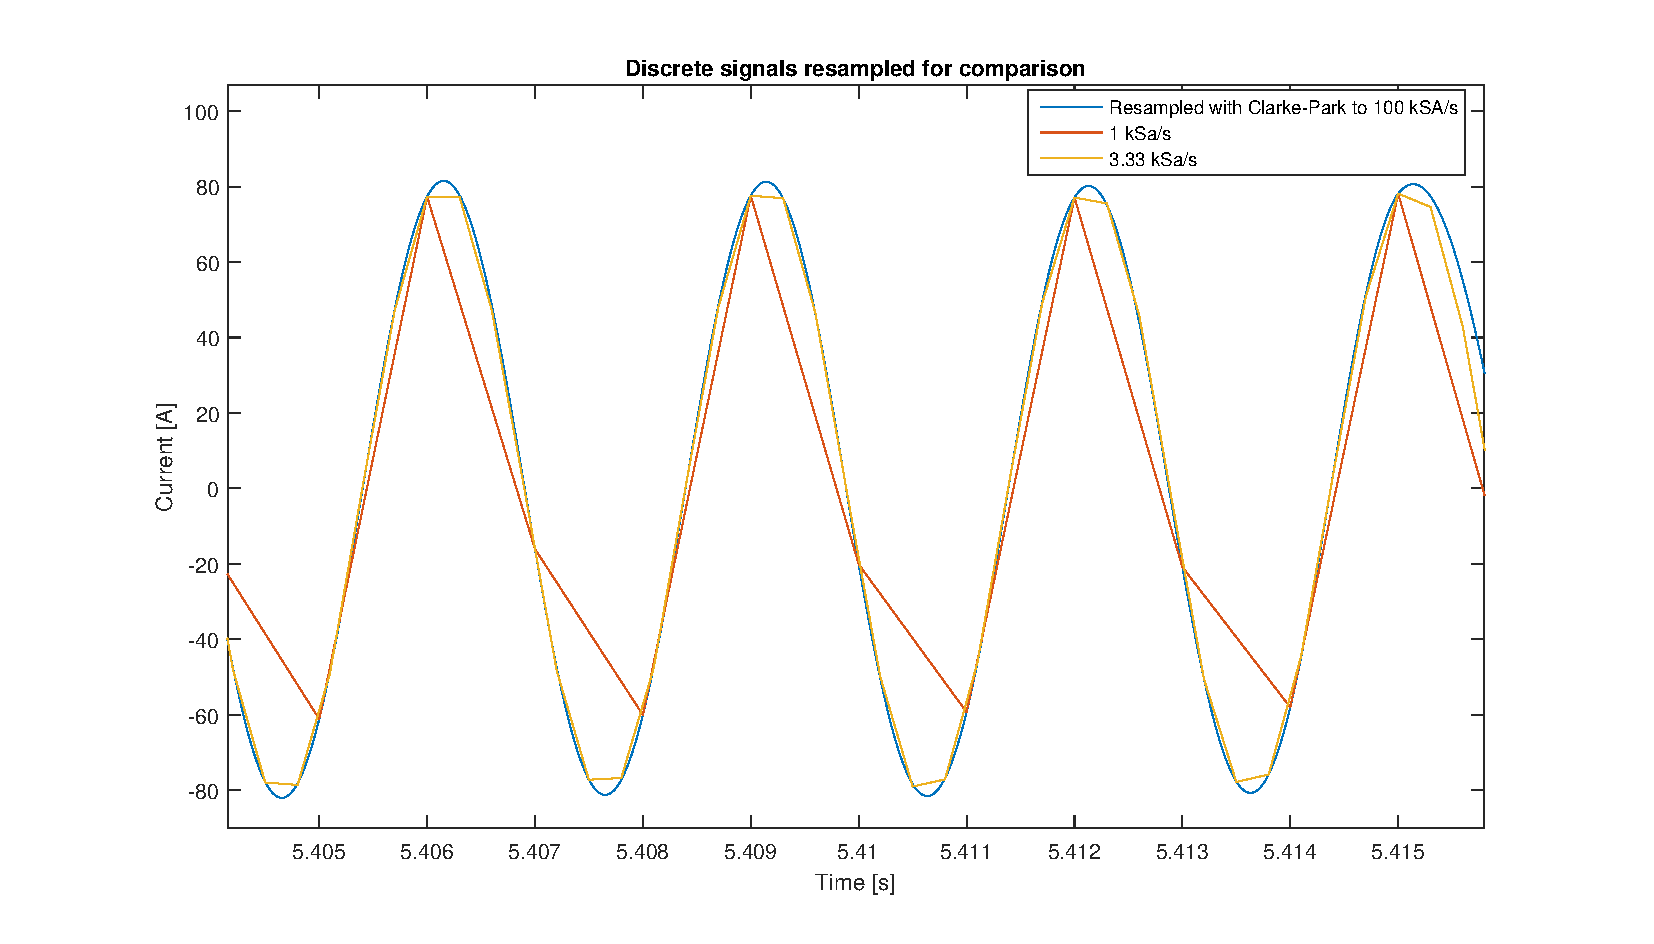
\includegraphics[width = 0.9\linewidth]{graphics/Clarke-park_resampled}	
	\caption{Comparison of data recorded at 1 kSa/s and 3.33 kSa/s, against 100 kSa/s resampled using Clarke-Park}
	\label{fig:Clarke-park_resampled}
\end{figure}

The resampled data from the 1 kSa/s and 3.3 kSa/s (orange and purple respectively on figure\ref{fig:Clarke-park_resampled}) are almost identical.
However, there is a small visible difference around the time 5.527 s, likely due to the limited precision of the encoder.
This also doesn't take into account any disturbance or noise, which could make it hard to reconstruct the signals with lower sample rates.\\

Additionally, the Matlab function, resample, produces nicely filtered vectors with smaller time steps, so it is possible to use a low sample rate for time invariant signals.\\
Another way to look at this is to calculate the maximum change in current from one sample to another.
This is determined by the inductance of the motor, which is $600 \si{\micro \henry}$ \todo[inline]{when one half bridge is high, and the two others are low, it's one armature inductance of 400 uH in series with two parallel armature inductances}, and the maximum voltage across it, which is $V_{BAT}=52.8 \si{\volt}$. 
At a sample rate of 3.33 kSa/s, this results in a theoretical maximum step of $264\si{\ampere}$.
A sample rate lower than this, would make it hard to properly record such sudden steps.

\subsubsection{Data Type}
When the sample rate is known, it is possible to get an estimate of how much storage space would be needed. 
It would be easiest, and most useful, to record using simple comma separated files, but these tend to take up more space than necessary.
The analog input to the Zybo are 12 bit, which means, that full precision of these would be possible with 4 digits, and often a decimal point and potentially a negative sign.
Including the horizontal separator, this comes to 6.5 bytes per point.\\

An example of recording could include time, two currents, a voltage and the encoder output, as displayed below
\begin{lstlisting}
Time	Ia	Ib	V	Encoder
1.0000	052.3	-278.1	52.56	16
1.0003	057.7	-280.4	52.54	17
\end{lstlisting}
That brings each line length to 32 bytes (8 bytes for time, 5.5 for the three analog, 3 bytes for encoder, 5 for separators).
At a sample rate of 3.33 kSa/s, this comes to 6.1MB per minute. 
With the current SD cards having 4 GB of free un-partitioned space, this gives up to 11 hours of recording time.\\

Alternately, it is possible to invent a file structure, that allows several arrays of with different data types.
By storing numbers in binary files instead of text, it is possible to reduce the space requirements to a third (2 bytes per analog, 4 bytes per timestamp (allowing up to 49 days of ms), and 1 byte for encoder).
This however will reduce the readability greatly, and include the workload, as one will need to write code both for encoding and decoding the file. \\

Since this is out of the scope of this project, and the sample rate isn't larger than it is, logging in standard ASCII will suffice.
Likely, different sample rates will be recorded to different log files









\subsection{Data Collection}
\label{sec:data_collection}
As described earlier there needs to be several sensors on the system in order to measure relevant parameters.
It should also be possible to add sensors at a later time by other developers. 
One micro-controller could be used for all sensors, but it would not be feasible when the numbers of sensors grow. 
The micro-controller would not have enough I/O peripherals to accommodate a lot of sensors. 
It might also not have the needed computational power. 
\\
Therefore a network needs to be realized. Each node in the network being a micro-controller and one or more sensors.
All sensor data needs to be collected by a node that transfers it wirelessly to the stationary computer.
This node will also need to log data as this eases the task of transferring log data to the stationary computer.
This node will be referred to as the wifi node.

\subsubsection{Network Topology}

There are various network topologies that can be used to setup the required node network for this project.
These include the ring-, bus-, mesh-, star- and tree-network topology. 
Before choosing a topology, a brief description of the purpose and functionality of the network as well as an overview of their advantages and disadvantages are needed. 

\paragraph{Purpose of the Network}~\\
\todo{Add the abbreviation ov = on-vehicle somewhere somehow}
The purpose of this network is to accommodate multiple nodes, such as sensors sub-networks and in general data-producers.
These nodes need to be able to transfer their data and receive massages from the wifi node.

The reasons for this is, that the use cases specify that sensor data should be transferred wirelssly and it needs to be possibly to start and stop specific nodes.
\\\\
The communication between the various nodes and the wifi node does not require a central hub.
Furthermore, in the case that one node fails, the network as a whole should still be operative.
Since it is a multi-node network and it may require more nodes in the future, scalability is also required.

\paragraph{Different Topologies}~\\
\todo[inline]{Thomas: This section needs to be cleaned of any statements such as "this is the simplest and cheapest...". They are broad conclusions that we have no merrits on saying}
\begin{itemize}
\item \textbf{Bus:} This is the simplest and cheapest topology.
All nodes communicate through a central bus and it is scalable with the addition of extra nodes on the two ends of the cable.
The central bus introduces the risk of complete network failure in case of the bus failure and the decrease in performance in case of many nodes or heavy traffic.
\item \textbf{Ring:} All the nodes in this type of network form a ring, where each node is connected to its two neighbors.
It has the advantages of the bus network as well and it shows better performance, even under heavy load.
A centralized control is not required for this type and in case of a node failure, the ring breaks and it can continue to function as a bus network.
It is scalable, but to a less extent than the bus.
\item \textbf{Mesh:} In this type, each node has direct connections to each other node present in the network.
That provides speed and reliability in case of node failures, but requires more hardware and processing power to manage the connections.
It is very robust but scalability is certainly not one of its features.
\item \textbf{Star:} The star topology is a centralized type of networking.
All nodes are connected to a central hub, handling all the communication between them.
It is fast, easy to implement and offers great reliability in case of node failures.
The major disadvantage is that if the hub fails, the entire network fails.
It can be scalable to a certain point, since the hub can be upgraded to handle more connections.
\item \textbf{Tree:} The last type, the tree is an extension of the bus and the star topologies combined.
It can be easily scalable, but that adds extra difficulty in its maintenance.
It also requires a lot of connections and in case the top (root) node fails, then all the network is down as well.
\item \textbf{Hybrid:} The last type is the hybrid one, where depending on the needs and purpose of the network, two or more topologies can be combined to achieve the best balance between their advantages and disadvantages.
\end{itemize}

\paragraph{Suitable Topology}~\\
For the systems networking purpose, the mesh type is not suitable, since it adds extra hardware requirements such as processing power and many redundant connections.
A node may be a simple sensor with a small micro-controller and hence, connecting it to such a network is not feasible.
%In our system, a small embedded board computer will be the ov-computer which requires to maintain its connection with the network even in case of failures and also possibly the central hub in centralized topologies that such as the star and the tree.
The star network requires a lot of connections which normally are not present at standard micro-controllers.
%Thus, these two topologies are not suited, since in case of its failure, the whole network fails.
Thus, the mesh and star networks are not suited for this system
Scalability is also a requirement for the future connection of nodes.
Although the majority of the types provide a level of scalability, the addition of extra nodes always decrease the overall performance of any network.
Hence, a topology that balances the decrease in performance against the network's expansion is best suited for the project.\\\\
The approach that fits the requirements is implementing a bus network, where each node may be a subnetwork of a different type depending on the needs, making it into a hybrid network having a bus topology as its basis.
This type provides a good balance of reliability, scalability, hardware requirements and communication speed in comparison to the others.

\subsubsection{Networking technology}

\paragraph{Existing Technologies}~\\
Different networking technologies exist in use today, such as Ethernet, CANbus, CANopen and Powerlink, among others.
CANbus is widely used in the automotive industry with data rates up to 1Mbit/s for small networks lengths, but the classic Ethernet and Powerlink support data rates of at least 10Mbit/s.
Furthermore, Powerlink is suitable for transmission of time-critical data and timing-synchronization of the nodes and CANopen networks are very robust and reliable.
\paragraph{Choosing a Technology}~\\
\todo[inline]{Mikkel: Remove were..}
The two choices that were considered for the scope of this project were Powerlink and CANopen.
The first one can be implemented using openPowerlink at a software level and utilizing PmodNIC100 modules provided by the university.
On the other hand, CANopen can be implemented using CANopenSocket\footnote{https://github.com/CANopenNode/CANopenSocket}, an open source git project built on CANopenNode.
This library is easily implemented in Linux and can use various hardware, one of them being a USB to CAN interface board named USBtin\footnote{http://www.fischl.de/usbtin/}.
Another available module to use is the CANbus.
Since CANbus is a technology widely used in the automotive industry, it is chosen for this system.



\subsection{CAN-bus}
The CAN (Controller Area Network) protocol was originally developed in the 1980's by Bosch.
It is a multi-master network, where each node connects to a common bus.
All nodes are able to broadcast data to all other nodes.
The CAN protocol includes an overhead of 47 bit per message.
The data sent in a message can vary in size from 0 to 8 bytes.
This is described in detail in section~\ref{sub:CanMessageFrame}.
The bus offers 1 Mbit/s on a bus of up to 40 \si{\metre} of length.

\begin{figure}[h!]
	\centering
	\includegraphics{graphics/canbus_setup}
	\caption{CAN node architecture}
	\label{fig:canbus_setup}
\end{figure}

Some hardware is necessary in order to properly realise a CAN network.
The structure of each node can be seen on figure~\ref{fig:canbus_setup}.
The following paragraphs explain the physical parts of this structure as well as the requirements of the protocol.

\todo[inline]{Thomas: My understanding of our protocol is that we are just interpreting the CAN messages in a different way. Do we actually need a detailed explanation of the actual CAN protocol?}
\todo[inline]{Thomas: Split this entire section into paragraphs, one for each (meaningful) box in figure~\ref{fig:canbus_setup}}

\paragraph*{The CAN Bus}~\\
The bus is shown on the bottom of figure~\ref{fig:canbus_setup}.
It is a differential signal bus.
This means that the value on the bus is determined by the difference of the two wires, rather than the absolute value of either signal.
The bus has to be made of twisted pair wires with a characteristic impedance of $\si{120 \ohm}$ and terminated at each end with a $\si{120 \ohm}$ resistor.
That means, that if the bus is broken at any point, no communication will work, even if two nodes are still connected.
Alternatively, it is possible to terminate each node, but this greatly reduces transmission speed.\\
\todo[inline]{Mikkel: Not sure I understand it.}
\paragraph*{The CAN Transceiver (XCVR)}~\\
The transceivers translate a Tx voltage signal to the differential CAN signal, and simultaneously translates the bus signal to Rx voltage signal. 
For this reason, it is not possible to implement this in most if not all microprocessors.
Because the CAN bus is differential, a transceiver would be able to read the signal it's putting out itself, but they do not transmit these to the Rx pin of the controller.
Other than this blocking of its own signal, it will translate whatever the controller puts out with.
CAN transceivers are reasonably simple in design and while they can be procured, it was decided to create a custom transceiver.
\todo[inline]{Mikkel: Above section is confusing for me.}
\todo[inline]{Thomas: And me too, The actual role of the xcvr is not clear from the text.}
\todo[inline]{Thomas: What analysis resultet in us deciding to build our own? Is this the right place for this decision?}

\paragraph*{The CAN Controller}~\\
This element can be standalone hardware, but it is in many cases built into the micro-controller.
The major advantage of having the controller built into the micro-controller is that it would not otherwise require another protocol to communicate between the microprocessor and controller.
\todo[inline]{Thomas: You mean that you would have to communicate with the controller through I2C, UART or w/e?}
The controller has an input and an output FIFO, meaning that the CAN bus communication operates asynchronously. 
This is necessary as there is only one bus and it is likely that there will be a queue of nodes trying to write to the bus.

\paragraph*{Protocol}~\\
The protocol in this case refers to a protocol running on top of CAN.
CANopen is a widely used protocol made specifically to expand on the usability of CAN.
The SevCon gen4 used on the go-kart utilises CANopen in its communication.
This makes CANopen a reasonable option to employ generally across the network.
CANopen is, however, quite complex and implements many features which are not needed in the monitoring system being developed.
Using CANopen would complicate greatly, the task of learning how to add new nodes to the system.
Another option is to design a protocol that fulfills the requirements,
\todo[inline]{Thomas: Are the requirements of the protocol actually outlined at this point?}
\todo[inline]{Thomas: At this point it needs to be clear that we want some scalability in the system, enabling us to add up to n (yes n, not 16), nodes. We may need to move figure \ref{fig:analysisnodes} to some other place.}
while still maintaining a simple structure.
As is shown on figure \ref{fig:analysisnodes}, it should be possible to add up to $n$ nodes.
This requirement should be considered in determining the design of the protocol.

\begin{figure}
	\centering
	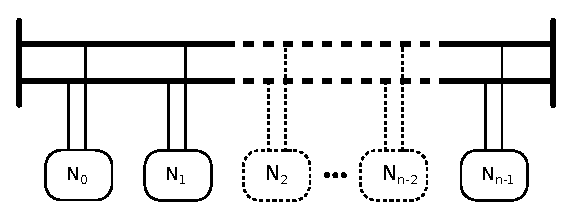
\includegraphics[width=.75\linewidth]{graphics/analysis_nodes}
	\caption{Overview of the network structure.}
	\label{fig:analysisnodes}
\end{figure}

The design of this protocol will be described in more detail section~\ref{sub:CAN_protocol}.\\







\todo[inline]{Thomas: Section describing the requirements of the structure and what requirements that would that result in in terms of the protocol}

\subsection{Micro-controller}
As described in section \ref{sec:data_collection} there should be a CAN network of nodes on the go-kart.
Each node is a sensor or other data producing unit along with a micro-controller.
From the perspective of the network the only requirement for the micro-controller is that it has a CAN controller.
In principle the network could consist of 16 different micro-controllers.

\subsubsection*{Sensor Nodes}
As described in section \ref{sec:hardware_for_par}, it was chosen to use an IMU and a GPS with a USB interface. 
As specified in the use cases one of the nodes needs to transfer data wirelessly from the go-kart to the stationary computer. 
Both USB interface and wireless data transfer drivers are implemented in operating systems like Linux, Mac OS X and Windows.
Thus choosing a micro-controller supporting such an operating system will greatly simply the code that needs to be written for those sensor nodes.
Developing software for Linux is a part of a course that the group is attending therefore Linux will be used as the operating system.
\\
The Zybo board will be used for the sensor nodes as it has a built-in CAN controller, it has the ability to run Linux and the group has access to it.

\subsubsection*{Zybo Board}
The Zybo board has a Xilinx Zynq Z-7010 chip, which has a processing system (PS) part and a programmable logic (PL) part.
The PS consists among other of a dual-core ARM Cortex-A9 processor and I/O peripherals including CAN and USB.
The PL consists of a Xilinx 7-series Field programmable gate array. 
The PL and PS are connected through a bus called AXI.
The Zybo board itself is a developing platform consisting, among other, of several buttons, switches, LEDs and connections for USB, Ethernet, HDMI and several PMOD connectors.


\subsubsection*{Linux on the Zybo Board}
Several Linux distribution are configured to run on the Zybo board. 
The group has experience with a the Xillinux \footnote{http://xillybus.com/xillinux} distribution, therefore this will be used.
Xillinux is based upon the Xilinx distribution which is based upon Ubuntu 12.04.
In the Xillinux architecture there is a bus between the PL and PS named Xillybus.
Xillybus is implemented as an IP core in PL and a corresponding Xillybus driver in the Xillinux kernel.
In PL the IP core is interfaced through standard FIFO buffers and the Xillybus is reached in userspace through \textit{"/dev/xillybus\_"}.
\todo[inline]{Mikkel: Check this path on Zybo.}

\subsubsection*{Conclusion}
Nodes on the network need not to be a specific micro-controller, they just need to able to use CAN.
The Zybo board running Xillinux will be used for IMU, GPS and wireless network node to ease development as Linux includes both USB and network drivers. 



















\subsection{Wireless transmission}
The wireless transmission between the go-kart computer and the stationary computer could be a number of different technologies.
This section seeks to find an appropriate one.

\subsubsection{Range}
The range of the transmission is determined by the length of the test track. 
Normally the SDU kart is tested on parking lots with a maximum lenght of 50m and width of 20m.
There are almost no obstacles for the transmission on such a parking lot. 
This test track sets a minimum requirement that the wireless setup should be able to transmit data at 55m with no obstacles.
\\
At some point it would be interesting to test the go-kart on a real go-kart track. 
The nearest go-kart track is \textit{Odense gokart Hal}, which is also thought to be an average indoor go-kart track.
The track is about 70m long and 40m in width with no obstacles other than the barriers. 
If the wireless transmitter and receiver are placed above the barrier then they will not an obstruction on the transmission. 
This track sets a minimum requirement of 80m transmission. 

\subsubsection{Speed}
The transferred data is from xx sensors producing a maximum of yy bites per sample. 
Data is only used for human inspection and therefore a sample frequency of 100Hz would be sufficient.
This gives a minimum requirement for the speed of the transmission to be ZZ Mbit/s. 

\subsubsection{Compatibility}
It should be possibly to change the stationary computer and therefore the chosen wireless transmission technology should be compatible with standard computers running linux.
The chosen hardware should be compatible with standard linux computers and the Zybo board. 
Both have USB ports and Ethernet ports as a standard, therefore the chosen hardware should one of those.

\subsubsection{Technologies}
Bluetooth is a technology that is compatible with standard computers running linux. 
Bluetooth 5.0 has a maximum speed of 50Mbit/s, which is sufficient.
The range of typical class 2 Bluetooth device is 10m \footnote{https://en.wikipedia.org/wiki/Bluetooth}.
This range is definitely not enough for this application.
\\
\\  
WiFi is also compatible with standard computers running linux and typical WiFi units has speeds that is a lot higher than the required. 
WiFi can be operating in the 2.4GHz band and in the 5GHz band. 
2.4GHz units has the highest range. 
The 802.11n protocol generally has the best range compared to the other 802.11 protocols \footnote{https://en.wikipedia.org/wiki/IEEE\_802.11\#802.11n}.
\\
A local network between computers without connection to existing networks such as the internet is referred to as an ad-hoc network. 
It is a required that the found hardware is capable of doing an ad-hoc network.

\subsubsection{Conclusion} 

\begin{table}[]
\centering
\caption{Minimum requirements for wireless transmission.}
\label{tab:req_wifi}
\begin{tabular}{|l|}
\hline
80m transmission range       \\ \hline
ZZ Mbit/s                    \\ \hline
802.11n protocol             \\ \hline
USB or Ethernet              \\ \hline
ad-hoc network compatability \\ \hline
\end{tabular}
\end{table}
Based on the requirements in table \ref{tab:req_wifi} it was chosen to us the TP-LINK TL-WN722N, as it uses the 2.4GHz band, the 802.11n protocol, is compatible with linux, has an external antenna and uses USB. 






















\subsection{Software on stationary computer}
There needs to be a user interface on the stationary computer to let the user monitor the go-kart parameters and start/stop sensors. 
This UI needs to present data in a graphical interface to ease the users "understanding".. Aaarh. Need.. Better... Words... 
\todo[inline]{Mikkel: better words.}
Different sensors will be added to the system continuously  
This means that the software on the stationary computer needs to be expandable and that there should be developed a generic way to access the go-kart data.
The generic structure should be similar to that of figure \ref{fig:setup_ui}.


\begin{figure}[h]
	\centering
	\includegraphics{graphics/UI}
	\caption{UI.....}
	\label{fig:setup_ui}
\end{figure}

\subsubsection*{Simple UI}
To develop a sophisticated graphical user interface is not the focus of this project and will therefore be omitted, but a simple UI should be implemented to give the system the wanted functionality shown in the use cases.
It could be a command line UI giving the user the 

\subsection{Local Storage}
Somewhere this should be answered!

How should local data storage be realised?

	


% section system_analysis (end)
\newpage
%!TEX root = ../main.tex
\section{System Requirements} % (fold)
\label{sec:system_requirements}

\martin{The big system picture should be on its own page}

\begin{figure}[!h]
	\centering
	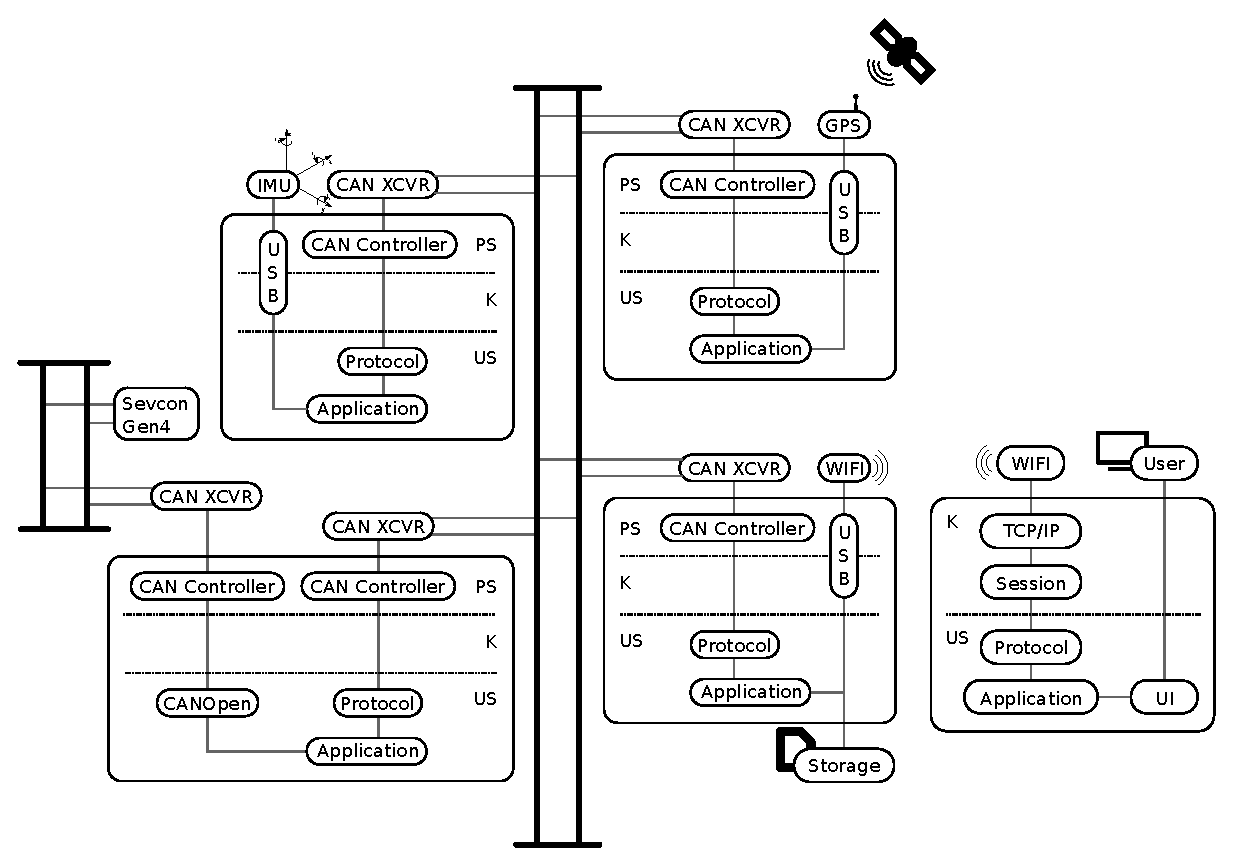
\includegraphics[angle=90,width=\textwidth]{graphics/analysis_complex.eps}
	\caption{The big system........}
	\label{fig:complete_system}
\end{figure}



\subsection{Actors}
The only actor on the system is an engineer.

\subsection{Interfaces}
\begin{itemize}
\item Wifi, for data transfer between go-kart and stationary computer.
\item CAN bus, for local network.
\item CanOpen, for interfacing the Sevcon.
\item USB, for GPS and IMU.
\item ??, for SD card connection.
\item Powersupply, for Zybo boards.
\end{itemize}

\subsection{Functional requirements}
The system: 
\begin{itemize}
\item Reads data from sensors.
\item Reads data from Sevcon.
\item Transfers data to stationary computer using Wifi.
\item Presents data to the user.
\item Logs sensordata to SD card.
\item Read data from SD card.
\item Timestamps all data. 
\end{itemize}

\subsection{Operational requirements}
The system monitors go-kart data.% when engineer starts the system by powering it on.

\subsection{Quality of service requirements}
\begin{itemize}
\item IMU data must be sampled with xx Hz.
\item GPS data must be sampled with zz Hz.
\item Data logging with qq Hz.??
\end{itemize}

\subsection{Parametric requirements}
Wifi range must be greater than xx meters.

\subsection{Design requirements}
The system:
\begin{itemize}
\item must be scalable to at least 16 sensors/nodes.
\item must be modular to allow easy integration of new sensors/nodes.
\item must be functional if one or more sensors/nodes stop working.	 
\end{itemize}


% section system_requirements (end)
\newpage
\part{Implementation}
%!TEX root = ../main.tex
Throughout the analysis a number of decisions were made regarding the hardware and technologies to be used in the realisation of the system.
These are outlined in section \ref{sec:analysisconclusion}.
It was found that it is necessary to implement two different networks, one for collecting the data on the go-kart and one for transmitting the data to a monitoring station, assumed to be a standard PC throughout the remainder of the report.
These two networks will be referred to as the on-vehicle and off-vehicle networks, respectively.
The implementation of these, along with the remainder of the system, is described in this part.
Should a user or developer wish to implement their own node, a guide exists in appendix \ref{app:addnode}, outlining the steps necessary to implement a node.

\thomas{I am not sure about this introduction, it seems very strange..}
\section{On-Vehicle Network}
%!TEX root = ../main.tex

\section{CAN bus}\label{sec:CANbus}
The CANOpen protocol runs on the CAN bus.
It was originally developed in the 1980's by Bosch.
It is a multi-master network, where each node connects to a common bus, and any node is then able to broadcast data to all other nodes.
The bus offers 1 Mbit/s on a bus up to 40 m of length. \todo{Martin: is this with or without the substantial overhead?}

\subsection{Physical Layer}\label{sub:CANphys}
The physical layer has three main parts: The CAN controller, the CAN transceiver and the bus itself. \\

The CAN controller can be implemented as a standalone IC, or in many cases integrated in the node itself.
The Zybo supports CAN, and an IP core is available, so the CAN controller is already given.\\

The CAN transceiver is connected to the controller by RX and TX voltage signals, and connects to the bus through two differential ports. 
The transceiver must support the standard ISO11898-2, as this is what the Sevcon motor driver uses.
The device SN65HVD232 from Texas instruments support this standard, and is supplied with 3.3 V, so it can be plugged right into the Zybo, and still communicate with the Sevcon even though its CAN bus uses $\si{5 \volt}$.
According to TI itself\cite{3.3V_CAN}, this family of $\si{3.3 \volt}$ transceivers are compatible and interoparable with other \si{5 \volt} transceivers, so long as they support the same standard.\\

The bus has to be made of twisted pair wires with a characteristic impedance of $\si{120 \ohm}$, and terminated at each end with a $\si{120 \ohm}$ resistor.
That means, that if the bus is broken at any point, no communication will work.
Alternately, it is possible to terminate each node, but this greatly reduces transmission speed, and will not be done.//

The transceivers have been mounted on boards, that plug directly into the Zybo's 12-pin PMOD connector, which will be stacked on top of each other. 
The schematic is shown below.

\begin{figure}[h!]
	\centering
	\includegraphics[width = 0.7\linewidth]{graphics/CAN_Schematic}
	\caption{Schematic of the two can transceivers. One board is build for two transceivers each with pads for termination}
	\label{fig:CAN_Schematic}
\end{figure}

The board has been designed to use the MIO ports, available in the PMOD JF. 
This is necessary to utilize the build in CAN controllers on the PS part of the Zybo.
Although the schematic contains two transceivers and two termination resistors, most of these devices are not mounted. 
Four boards will be made, all containing CAN0, C0 and the ZYBO connector. 
One board will also include the resistor R0 - this is the bottommost board
Another board will include R0, R1 CAN1, C1 and the SEVCON connector.
Ths is placed on top, to allow the SEVCON connector's screws to be accessible. 
The stack is visible below

\begin{figure}[H]
	\centering
	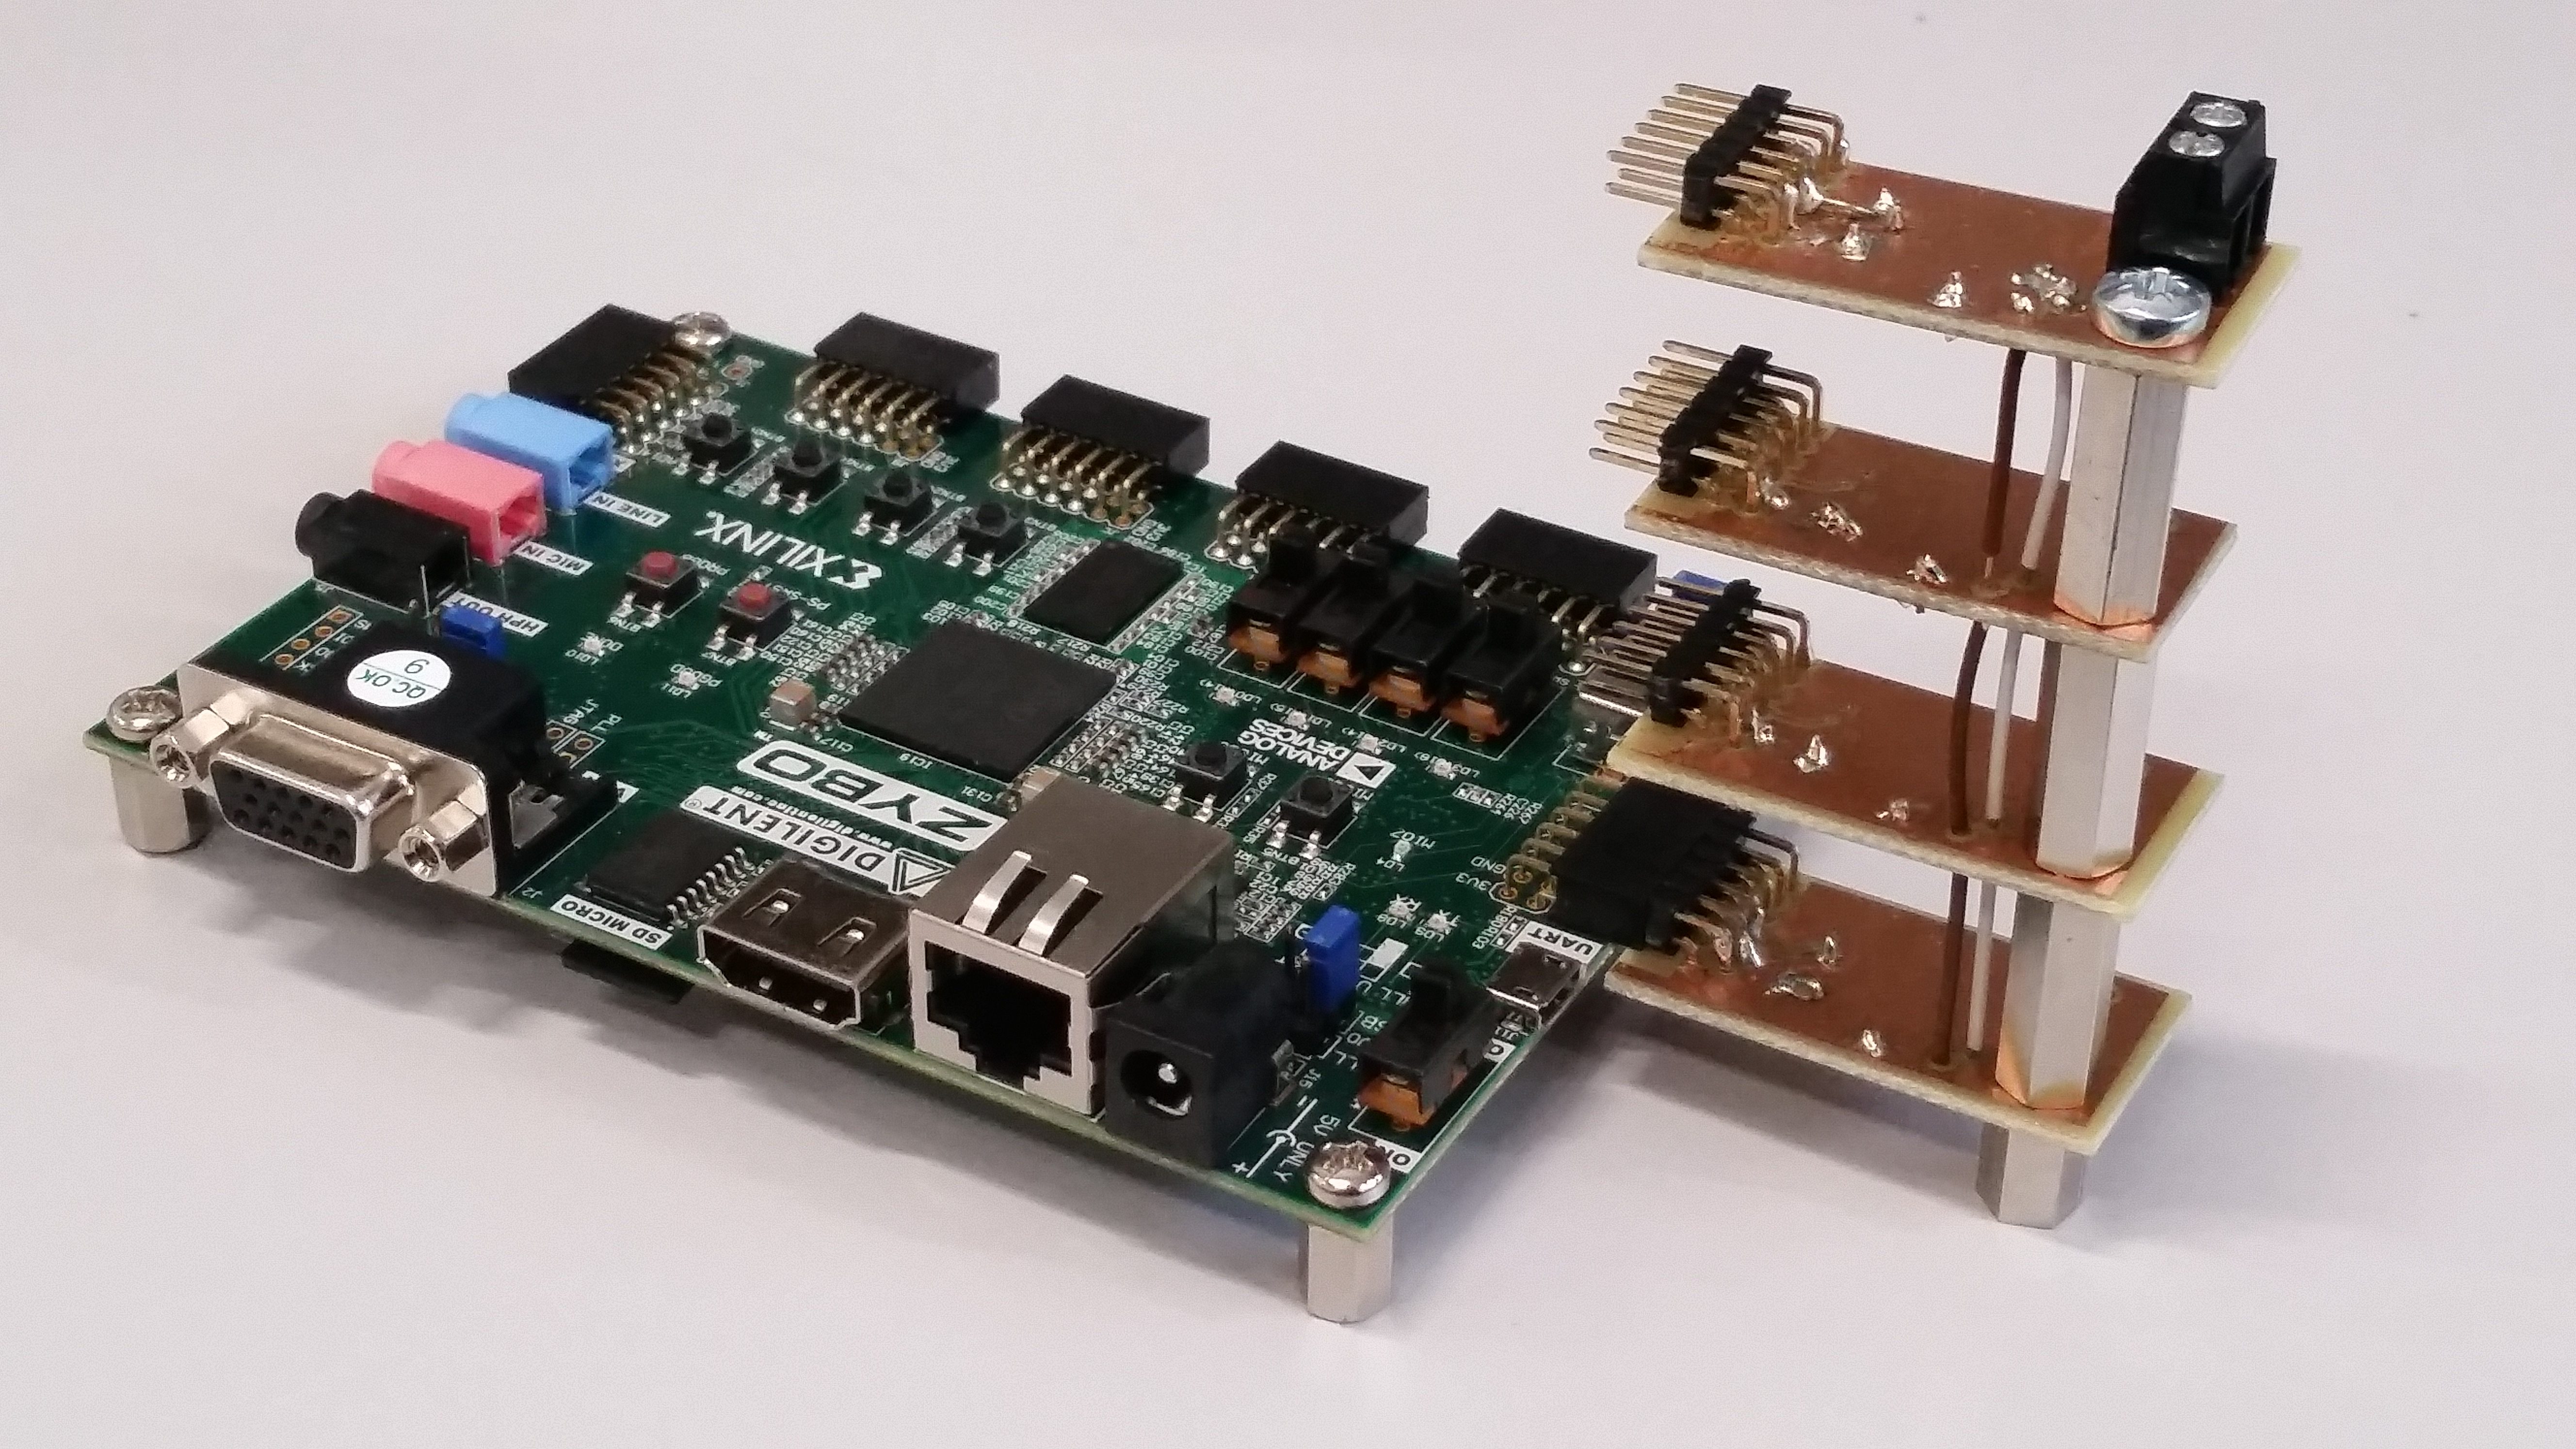
\includegraphics[width = 0.9\linewidth]{graphics/CAN_stack_picture}
	\caption{The CAN stack plugged into one Zybo}
	\label{fig:CAN_stack_picture}
\end{figure}

\subsection{Implementation of the Physical layer}\label{sub:CANphys_implementation}
The Zybo has two build in
\todo{I suppose you want to say built-in}

\subsection{Testing the CAN stack for a basic network}
After the design and printing of the stack board, testing it was the next step.
The test included using one the CAN controllers within the Zynq chip with the purpose of showing that a basic CAN network between two Zybo boards could be implemented using the stack.
Specifically, the one Zybo was sending the input value of the buttons to the network in order to be received by the second one and turn on the on-board LEDs as a result.
After designing a basic architecture in Vivado and writing a source code, the test was successful, thus proving the basic functionality of a CAN network.
All Zybo boards were programmed with the same architecture and source code.

\subsubsection{Architecture}
In order to realize the above test, enabling the CAN controller inside the Zynq chip as well as including two AXI GPIO cores were necessary. One AXI GPIO was setup as leds 4bits while the other one as btns 4bits as it can be seen in figure \ref{fig:CAN_Testing_Architecture}. 

\begin{figure}[h!]
	\centering
	\includegraphics[width = 0.9\linewidth]{graphics/Zybo_BasicTestingArchitecture_for_CAN}
	\caption{Block diagram featuring the testing architecture in Vivado.}
	\label{fig:CAN_Testing_Architecture}
\end{figure}

\subsubsection{Source Code}
%!TEX root = ../main.tex

\subsection{CAN protocol}\label{sub:CAN_protocol}
Due to the requirements of the on-kart network, it is decided to formulate a new protocol specifically for this project. The requirements are listed below.
\textbf{On-kart network requirements}:
\begin{itemize}
	\item Simple and easy to learn.
	\item Support for 16 nodes.
	\item Broadcast data.
	\item Defining message types.
	\item Variable data length - beyond 8 bytes per message
	\item Expandable.
	\item Commands: Start/stop broadcasting 
	\item Commands can be send to specific or all nodes
\end{itemize}

The basic CAN framework is retained for this protocol. 
The message ID is split in to two portions: The first four bits indicate the transmitting node ID, which will allow up to 16 nodes, all included. 
The last 7 bits of the message ID would contain an identifier for what the data portion of the frame contains.
Each node would then have a list of message IDs (11 bits), that it knows how to handle.
If a message is not on that list, the node will ignore it.
//
There are basically two types of nodes: The node containing with the Wifi link \todo[inline]{We should agree on names for the nodes, IE, Wifi node, IMU node and so on.}, and all other nodes.
Generally nodes can either produce data, and/or receive commands.
The Wifi node does neither produce any kind of data nor receive commands, but it odes receive data, and send out commands.
Therefore, there is a special case, for where the Wifi node is sending.
In this case, the subsequent four bits determines the recipient, leaving three bits for command type. 
For this part, command types are only "Start broadcasting" and "Stop broadcasting", but could be extended to for instance "Set parameter" or "Set value", where the data field will indicate which parameter, and what is's set to.



%!TEX root = ../main.tex
\subsection{Functions of the GoCAN Protocol}\label{sec:CAN_functions}
Some additional functionality is required in GoCAN to fulfill the requirements set.
This functionality is described throughout this section.

\subsubsection*{Timestamps}
As mentioned in section~\ref{sec:CAN-bus} the CAN protocol is not real time, therefore all data on the bus must be timestamped before transmission. 
The resolution of the timestamps has been decided to be 1 ms, as this leaves sufficient accuracy for the sensors analysed in this project.
This presents several challenges, in terms of what the time reference is and how to convey timestamps with adequate precision without creating too much overhead.
With internet access, the Epoch timestamp is available. 
This is infeasible in bare-metal code.
Instead a counter will be implemented on each node, incrementing an 32 bit integer every 1 ms.
This gives 49.6 days before overflowing.\\

Because a standard 32 bit integer takes 4 bytes, it would introduce a large overhead if the timestamp is sent with every message. 
Instead, each timestamp will determine the time of all subsequent data messages, until a new timestamp is sent. 
As an example, the pseudo code below describes the transmission of all nine axis of the IMU with the same timestamp.
Additionally, the IMU can transmit pressure and temperature measurements, but as these are slower signals, they would be transmitted at a lower rate.

\begin{lstlisting}
Send Timestamp
Send Ax, Ay, Az
Send Gx, Gy, Gz
Send Mx, My, Mz
Wait
Send Timestamp
Send Ax, Ay, Az
Send Gx, Gy, Gz
Send Mx, My, Mz
Send Pressure, Temperature
Wait
\end{lstlisting}

Lines 2-4 are measurements taken at the timestamp in line 1.
The WiFi node appends the corresponding timestamps to each of these nine data points with the corresponding timestamp.
Lines 7-10 refer to the timestamp at line 6.

\subsubsection*{Commands}
The WiFi node is capable of issuing commands on the network.
As described in section~\ref{sub:CAN_protocol}, it is possible to start and stop any specific or all other nodes from the WiFi node.

\subsubsection*{Synchronization}
Another specific command is the synchronization command. 
When the system starts all nodes will start polling their Rx FIFO for this sync command. 
When this command is received, the node will start the millisecond timer.

\subsubsection*{Multiframe Messages}
Due to the limited data length of a CAN frame, it is likely necessary to support multiple frames per message. 
Generally it is better to use all 8 bytes of data in one frame, to reduce the relative size of the overhead, and in case a dataset isn't easily split into 8 byte portions, it might be easier to bundle it all together and send as multiple full frames. 
In the message ID of all but the first frame of a multi-frame message the \texttt{new message}, to make it highest priority.
That way a message will not be interrupted by other messages from other nodes.
The construction and interpretation of these multiframe messages are described in sections~\ref{sec:sensor_node} and~\ref{sec:frontend}.

\subsubsection*{Datatype and Scaling}
As most sensor data comes from sources of limited resolution, the optimal solution would be to send only the number of bits that are measured. 
In some cases however that is not possible, and a better solution is to round up or down to the nearest byte, and send the data as a fixed point data type.
Intead of defining a new datatype, an integer of appropriate length will be used instead, and the object dictionary will define the scaling. \\

As an example, the message described in table~\ref{tab:message17_OD} contains four data points of 2 bytes. 
This contains the current measurements on the three phases along with the electrical position of the rotor.
An example is described in table~\ref{tab:message17_OD}.

\begin{table}
	\centering
	\begin{tabular}{l|l|l|l|l|l}
		Message ID & DLC & $\mathrm{I_a}$ & $\mathrm{I_b}$ & $\mathrm{I_c}$ & $\mathrm{\Omega _e}$ \\ 
		\hline
		10100001001 & 1000 & 414 & -1545 & 1131 & 13090 \\
		\hline
		 & & 25.9 A & -96.6 A & 70.7 A & 1.31 rad
	\end{tabular}
	\caption{Example of message data from line 17 of table~\ref{tab:OD}}
	\label{tab:message17_OD}
\end{table}
According to table~\ref{tab:OD}, there are two scaling factors defined, one for currents and one for angle. 
The bottom line of table~\ref{tab:message17_OD} shows the resolved measurements.

%!TEX root = ../main.tex
\subsection{Implementing CAN utilizing XCanPs}\label{sec:methods_to_implement_can}

\mikkel{DONE:move axi can to analysis.}
\mikkel{move assymetric multiprocesssing to future work}
\mikkel{ move bare metal first}
\mikkel{split from linux part.}
\martin{The can controllers do not have anything to do with xilinux. Does Xilinux provide drivers for the can controllers on the zynq? CAN controllers vs CAN drivers Issue - Some things rephrased.}

This section includes the process that was followed to enable the CAN controller in Linux.
The purpose of this was to gain access to the controllers from Linux.
Using this operating system was necessary for using the required USB interfaces, logging the data into files as well as utilizing the network tools to establish an ad-hoc network.
The steps for this were to modify certain files related to the kernel configurations and the device tree settings.

\subsubsection*{Enabling the CAN Controller Drivers}

According to Xilinx documentation, the process for enabling the CAN controllers on the Zynq7 Processing System, the Linux CAN driver guide \cite{Xilinx_wiki_Linux_CAN_driver} was needed to be followed.
Specifically, the Kconfig file under the path \ref{code:can_kconfig_pathfile} needed to be configured.
The entry at line 128 was changed as seen in code \ref{code:can_kconfig_contents_line128}.
Originally, lines 130 and 131 were as seen in code \ref{code:can_kconfig_original_line130}.

\begin{lstlisting}[caption={CAN Kconfig pathfile.},numbers=none,label=code:can_kconfig_pathfile]
/usr/src/kernels/3.12.0-xillinux-1.3/drivers/net/can
\end{lstlisting}

\begin{lstlisting}[firstnumber=128,caption={Kconfig file contents from line 128.},label={code:can_kconfig_contents_line128}]
config CAN_XILINXCAN
	tristate "Xilinx(*@ @*)CAN"
	depends on NET [=y] && CAN_DEV [=y] && CAN [=y] && 
        (ARCH_ZYNQ || MICROBLAZE [=y])
	default y
\end{lstlisting}

\begin{lstlisting}[firstnumber=130,caption={Original content of lines 130 and 131.},label={code:can_kconfig_original_line130}]
	depends on CAN && (ARCH_ZYNQ || MICROBLAZE)
	default n
\end{lstlisting}

The next step of the process was the modification of the device tree settings file, requiring an entry for the CAN PS to be inserted.
The necessary file was located under the boot folder named as seen in \ref{code:dts_file_zybo}.
The modifications can be seen in code \ref{code:dts_changes_zybo} for can controllers as well as for the AXI CAN core.

\begin{lstlisting}[numbers=none,caption={Device tree settings file and its path.},label={code:dts_file_zybo}]
/boot/xillinux-1.3-zybo.dts
\end{lstlisting}
\catalin{Double quotes are problem here as well. FIX THEM WHENEVER}
\begin{lstlisting}[caption={Device tree settings changes.},label={code:dts_changes_zybo}]
zynq_can_0: can@e0008000 {
        compatible = xlnx,zynq-can-1.0;
        clocks = <&clkc 19>, <&clkc 36>;
        clock-names = can_clk, pclk;
        reg = <0xe0008000 0x1000>;
        interrupts = <0 28 4>;
        interrupt-parent = <&intc>;
        tx-fifo-depth = <0x40>;
        rx-fifo-depth = <0x40>;
    };
axi_can_0: axi-can@40000000 {
        compatible = xlnx,axi-can-1.00.a;
        clocks = <&clkc 0>, <&clkc 1>;
        clock-names = can_clk,s_axi_aclk;
        reg = <0x40000000 0x10000>;
        interrupt-parent = <&intc>;
        interrupts = <0 59 1>;
        tx-fifo-depth = <0x40>;
        rx-fifo-depth = <0x40>;
        };
\end{lstlisting}

Unfortunately, the above steps did not enable the drivers successfully.
After the changes, the CAN devices were still not visible in Linux and thus, connection to the CAN network was not feasible.
Research was done by the authors in why this could not be accomplished.
It was found that there were some naming inconsistencies between the guide and the Device Tree Settings file present in Linux running on the Zybo. Specifically, all the devices' names in the file are prepended with ps7.
A new set of changes with this naming convention was done, but with no success.\\

The files mentioned above were modified in the Linux running on the Zybo.
It was expected the changes to take effect after rebooting the system, which was not the case.
Another approach to this, was to build a new kernel containing these changes and to entirely build a new Linux system for the Zybo.
This proved to be unachievable because of the various patches that had been applied to the initial kernel by Diligent Inc. and Xilinx.
A new updated kernel with those patches could not be built MIKKEL.
\mikkel{say a few words why could not be built, just the main reason, after ...could not be built ....}

%The architecture can be seen in figure \ref{fig:CAN_Arch_with_AXI_CAN}.

%\begin{figure}[h!]
%	\centering
%	\includegraphics[width = 1.2\linewidth]{graphics/Zybo_Arch_with_AXI_CAN.png}
%	\caption{Block diagram featuring the architecture in Vivado with the AXI CAN core.}
%	\label{fig:CAN_Arch_with_AXI_CAN}
%\end{figure}


\catalin{Explain the code in more detail. Also mention the interrupt part for gpio.}
\subsection{CAN Controller Software}
\subsubsection{Implementation in code}~\\
As mentioned in section \ref{sub:Basic_SourceCode}, the code was based on the xcanps polled example available by Xilinx documentation.
The important functionalities that needed to be provided by the final software version included:
\begin{itemize}
\item receiving and sending of frames
\item creating the message id
\item decoding of the message id parts, such as the node id, the message type etc. \catalin{what else?}
\item handling button interrupts
\item controlling the LEDs
\item accepting and ignoring messages according to the subscriptions list
\end{itemize}
\catalin{What other functionalities? And, 1st letters capitals or not?}
The figure \ref{fig:SeqDiagram_SendFrame} shows the procedure of sending a frame to the CAN network containing data, which makes use of the protocol function createMsgID().
After returning the message id, the id and the data are put into the TxFrame to be sent once the FIFO has space.
The actual sending is done with a call to the XCanPs function XCanPs\_Send().
\\
Similarly, the procedure of receiving a frame is shown in the figure \ref{fig:SeqDiagram_RecvFrame}.
The node once it calls the RecvFrame() function, it waits in a loop until it receives a frame. Then, it checks the subscriptions in order to forward the packet for further processing or to ignore it.


This was achieved by implementing a set of functions and an array variable of subscriptions for each node.

\begin{figure}[h!]
	\centering
	\includegraphics[width = 1.1\linewidth]{graphics/SeqDiagram_SendFrame.pdf}
	\caption{The sequence diagram of the process of sending a frame.}
	\label{fig:SeqDiagram_SendFrame}
\end{figure}

\begin{figure}[h!]
	\centering
	\includegraphics[width = 1.1\linewidth]{graphics/SeqDiagram_RecvFrame.pdf}
	\caption{The sequence diagram of the process of receiving a frame.}
	\label{fig:SeqDiagram_RecvFrame}
\end{figure}

\begin{figure}[h!]
	\centering
	\includegraphics[width = 1.1\linewidth]{graphics/StateDiagram_CanStackTestCode.pdf}
	\caption{Behavioral diagram of the basic source code.}
	\label{fig:CAN_Testing_StateDiagr_Code}
\end{figure}
%!TEX root = ../main.tex
\subsection{Object Dictionary}\label{sub:OD}
In order to ensure that all message IDs are unique, an Object Dictionary is declared for this high level protocol.
The name is inspired from CANopen, but unlike the CANopen Object Dictionary, this refers to the messages being transmitted on the, and not the parameters or variables on the CANopen node.
Because of this, some variables appear in several message IDs, as it might be desirable to reconfigure some nodes to send different data, and the node should group data together to reduce the number of frames.\\

At this time, there are four nodes in the Object Dictionary with their node ID in hex: Wifi 0x1, IMU 0x3, Sevcon 0x7 and GPS 0xD.
The Wifi node is considered the master, and can command the other nodes, and as such it's portion of the OD is a bit different. 
Common for the other three nodes is that the message type 0x01 is a four byte timestamp.
Other than that, data messages start from 0x08.\\

Table~\ref{tab:OD} in appendix~\ref{app:OD} on page~\pageref{tab} contains the Object Dictionary in its current form.


\section{Off-Vehicle Network}
\label{sec:wifi}
%!TEX root = ../main.tex
\section{Networking}
The system deviced throughout this report seeks to ease the task of collecting data from the go-kart.
This is done by creating a network on the go-kart which allows the user to more easily add additional sensors.
In addition to providing a flexible platform for adding sensors, it will collect the data produced by the sensors on the network.
A goal with the project is to be able to monitor relevant data live through some interface.
To properly monitor data collected during driving it is necessary to maintain a live feed from the go-kart to the observer.
\\~\\
As mentioned above, there are two major functions to the system; recording of data and monitoring of data.
The recording is done on the go-kart using embedded hardware, specifically the Zybo platform is used to interface to the sensors.
The monitoring is done using a PC.
Monitoring is less time critical than the recording as it is simply meant for human readability.
For this reason, and to ease the workload, it has been decided to use a wifi connection between the go-kart and the PC.
Wifi, or even TCP/IP over ethernet is not viable on the go-kart between the Zybo boards due to the potentially long lag in that protocol.
A different network type will have to be devised for the embedded portion of the system.
This splits the network up into two parts, one that links the PC to the go-kart and one that links each component on the go-kart.
See figure \ref{fig:basic_network}.

\begin{figure}
	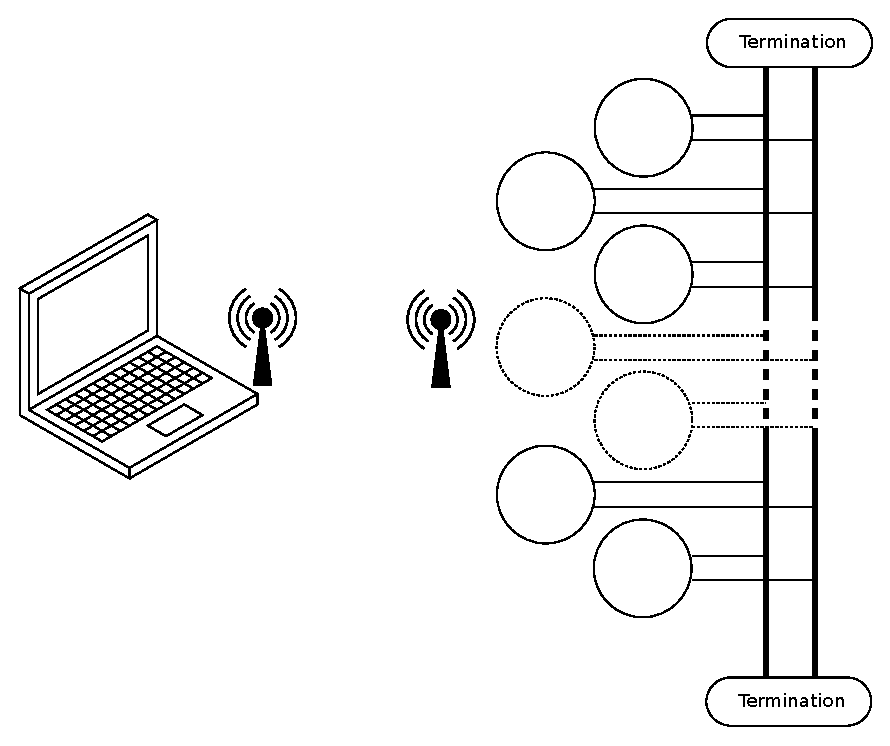
\includegraphics[width=.75\linewidth]{graphics/basic_network}
	\caption{A line of text}
	\label{fig:basic_network}
\end{figure}

These will be referred to as the off-kart network and the on-kart network, respectively, throughout the remainder of the report.
The following sections will explore the creation of both of these networks in turn.

\subsection{Off-Kart Network}
As mentioned above, the off-kart network is done using wifi.
It was chosen to use this method as all modern laptops are equipped with the capability of connecting to such a network.
Hereafter the challenge lies in establishing an ad-hoc network between a zybo board and a PC.
This network is created using the a USB-Wifi dongle on the Zybo board. 
The following script is run to bring down the device, change the network type to ad-hoc, bring up the device, create the ad-hoc network and, finally, assign an IP-address to the device.
\begin{lstlisting}
sudo ip link set wlan0 down
sudo iw wlan0 set type ibss
sudo ip link set wlan0 up
sudo iw wlan0 ibss join go-kart 2412
sudo ifconfig wlan0 192.168.10.9
\end{lstlisting}
It is verified working using the ping command from both the Zybo board and to the PC and vice versa.
Below is a thorough description of the challenges encountered while setting up this device as well as a brief explanation of the choice of device.
\\~\\
Two methods were immediately available for use: A usb wifi dongle and a PMOD wifi interface.
As the name implies, the latter is designed to be compatible with the PMOD interfaces on the zybo board (and a range of similar boards offered by Digilent Inc.).
It converts TCP/IP to SPI and vice versa.
However, since the zybo boards are already running a linux distribution, it was decided to attempt connecting through the usb wifi dongle.
This decision marked the beginning of a long journey, the highlights of which are discussed below. 
\\~\\
The first step was to ensure that the correct drivers are present on the system.
The usb dongle is a TP-LINK TL-WN722N.
This device uses the Atheros AR9271 chipset and is on the list of supported devices for the ath9k\_htc driver on wireless.wiki.kernel.org.
Running \texttt{dmesg} prints the kernel log, revealing, amongst other things, what drivers are loaded.
\begin{lstlisting}
dmesg | grep ath
[10.329564] usb 1-1: ath9k_htc: Firmware htc_9271.fw requested
[10.332438] usbcore: registered new interface driver ath9k_htc
\end{lstlisting}
Additionally:
\begin{lstlisting}
lsusb | grep Ath
Bus 001 Device 002: ID 0cf3:9271 Atheros Communications, 
	Inc. AR9271 802.11n
\end{lstlisting}
As per these commands the operating system (OS) has correctly detected and loaded the driver.
The \texttt{iproute2} package contains the utilities used to manipulate TCP/IP connections.
\begin{lstlisting}
ip link show
1: lo: <LOOPBACK,UP,LOWER_UP> mtu 65536 qdisc noqueue 
	state UNKNOWN mode DEFAULT group default 
    link/loopback 00:00:00:00:00:00 brd 00:00:00:00:00:00
2: eth0: <BROADCAST,MULTICAST,UP,LOWER_UP> mtu 1500 qdisc pfifo_fast 
	state UP mode DEFAULT group default qlen 1000
    link/ether 00:0a:35:00:01:22 brd ff:ff:ff:ff:ff:ff
3: wlan0: <BROADCAST,MULTICAST> mtu 1500 qdisc mq 
	state DOWN mode DEFAULT group default qlen 1000
    link/ether ec:08:6b:1b:41:b3 brd ff:ff:ff:ff:ff:ff
\end{lstlisting}
The device has been given the identifier \texttt{wlan0}.
It can be brought up by:
\begin{lstlisting}
ip link set wlan0 up
ip link show wlan0
3: wlan0: <NO-CARRIER,BROADCAST,MULTICAST,UP> mtu 1500 qdisc mq 
	state DOWN mode DEFAULT group default qlen 1000
    link/ether ec:08:6b:1b:41:b3 brd ff:ff:ff:ff:ff:ff
\end{lstlisting}
At this point the device is up, as can be seen on the list of flags:
\begin{lstlisting}
<NO-CARRIER,BROADCAST,MULTICAST,UP>
\end{lstlisting}
However, the \texttt{NO-CARRIER} flag is also set.
This flag indicates a fault on the physical layer, i.e. a disconnected network cable or similar.
In an attempt to isolate the error the dongle was connected to a PC.
The dongle worked flawlessly on the PC and connected to the internet after bringing down the standard interface.
Clearly, there are differences between the two systems, one or more of which were causing the 
Eliminating these differences 
\subsection{On-Kart Network}

\section{Nodes}
%!TEX root = ../main.tex
\mikkel{An introductiontion needs to be here!}
The designed network generally have two types of nodes, a generic sensor node and the wifi node.
This section will seek to design and implement software that adheres to the requirements listed earlier.
A node can be any kind of microcontroller, but this section will only address the case where a Zybo board is used. 

\subsection{Sensor Node}
\label{sec:sensor_node}
The requirements state that it should be simple to add new sensor nodes to the system. 
To realize this the node software should be designed to be modular.
It should be easily identified what software and what interface a developer of a new sensor node must adhere to.

An example of a node can be seen in figure \ref{fig:gps_node}.

\mikkel{Where to put this text?}

%The coming sections will explain the design of the node software that will provide the mentioned functionality using the design requirement.

\begin{figure}[!h]
\centering
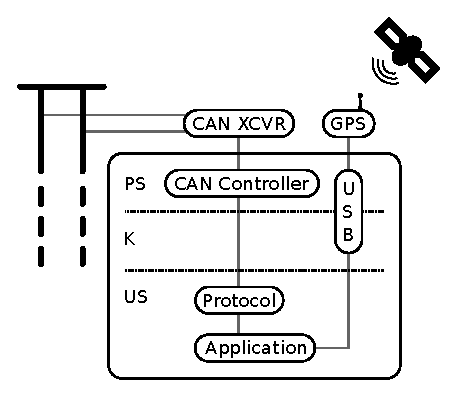
\includegraphics[width=0.5\textwidth]{graphics/analysis_gps.eps}
\caption{GPS node implemented on Zybo board.}
\label{fig:gps_node}
\end{figure}
\mikkel{Maybe change this figure to reflect the real system???}

This specific node has a GPS attached to it connected through a USB interface, but in general it could be any kind of data producing unit connected through any kind of interface.
\mikkel{How do we do this referencing nicely?}
From the requirements, table \ref{tab:requirements}, it is found that the sensor node software needs to fulfill requirements 1,2,6,10,11,12,20 and 21.
From the analysis section is it clear that a sensor node has the following responsibilities:

\begin{itemize}
\item Get data from associated sensor.
\item Pack data according to the specified protocol.
\item Construct CAN package
\item Send data using a CAN controller.
\item Get data from CAN network.
\item React to commands sent to it.
\end{itemize}

As described earlier the responsibility of sending data using a CAN controller and receiving data from the CAN network is done in the earlier described bare-metal code.
This section will focus on the designing and implementing code that provide the rest of the listed functionalities.

Analyzing on the procedure when data goes from a sensor to the CAN program resulted in the block diagram of figure \ref{fig:block_gps}.

\begin{figure}[!h]
    \centering
    \begin{subfigure}[b]{0.33\textwidth}
        \includegraphics[width=\textwidth]{graphics/FlowChart_Node_Packing}
        \caption{Ingoing data....}
        \label{fig:filter_full}
    \end{subfigure}
    ~
    \begin{subfigure}[b]{0.33\textwidth}
        \includegraphics[width=\textwidth]{graphics/FlowChart_Node_Unpacking}
        \caption{Two minu.}
        \label{fig:filter_2}
    \end{subfigure}
        \caption{Outgoing data.}
           \label{fig:filter_fulll}
\end{figure}
To design modular software it needs to be analyzed which blocks are the same for all nodes and which are sensor specific.
The sensor specific tasks are found to be extracting data from sensor and to pack data according to the protocol.
The remaining tasks are the same for all sensor nodes in the system. 
The procedure when data is going from the CAN program to the node is shown in figure \ref{fig:block_gps}.
All tasks are found to be generic for all sensor nodes.

\subsubsection*{Class diagram}
Based on the previous analysis a class diagram was developed and can be seen in figure \ref{fig:node_class_diagram}.
Classes to the right of the dashed horizontal is sensor specific and should be developed for each specific sensor.
Classes to the left are agnostic to all data they receive going from the sensor and to the CAN network.
They are generic classes and should be reused when developing new nodes.

\begin{figure}[!h]
\centering
\missingfigure[figwidth=1\textwidth]{Class diagram}
\caption{Class diagram showing node software.}
\label{fig:node_class_diagram}
\end{figure}

A struct containing all fields of a data packet in boolean data types is defined in listing \ref{code:data_packet}.  

\begin{lstlisting}[caption=Struct for data packet.,label=code:data_packet]
struct data_packet {
  std::bitset<1> sof;
  std::bitset<4> node_id;
  std::bitset<4> n_data_bytes;
  std::bitset<6> messagetype;
  std::vector<bool> data;
(*@\makebox[\linewidth][c]{$\smash{\vdots}$}@*)
};
\end{lstlisting}
It will be passed between the classes and they will each add their own information. 

The classes and their tasks from figure \ref{code:data_packet} will be explained here.

\mikkel{Put color explanation here?}

~\\ \par \textbf{GPS class} ~ \\
The GPS class needs to extract data from a connected GPS unit and update its own variables with that data.
The specific GPS unit used in this project has a USB interface and uses the NMEA protocol to format data.

~\\ \par \textbf{Packer\_GPS class} ~ \\
The Packer\_GPS class is also sensor specific and is the link between the sensor and the data agnostic node.
It is hard-coded with the message types that the sensor is allowed to send onto the network.
It has the responsibility to pack data according to the developed protocol.
Data in the form of a vector of booleans are then put into the \texttt{data\_packet} struct and passed to the node class.
The reason for making a separate class for the packer and not putting the functionality into the GPS class is that if the specification of the protocol or message types change, only this class needs to be modified.

~\\ \par \textbf{Node class} ~ \\
The Node class gets \texttt{data\_packets} from the Packer class it then needs to append its node id to it.
It needs to create a timestamp \texttt{data\_packet} each time data is to be sent.
In order to create the time message the class needs to keep track of milliseconds since last received synchronize message.
The class receives start, stop or synchronize events from the protocol class and reacts to those accordingly.

~\\ \par \textbf{Protocol class} ~ \\
The protocol class receives \texttt{data\_packets} from the node class. 
If it receives \texttt{data\_packets} where there are more than eight data bytes it needs to create additional \texttt{data\_packets} and distribute data to them. 
The additional \texttt{data\_packets} must have the same node id and message types, but the start of frame, sof, bit should be set accordingly.
The class also needs to append number of data bytes, \texttt{n\_data\_bytes}, to each \texttt{data\_packet}.
On \texttt{data\_packets} coming from the CAN network the class needs to use the last two bits of the messagetype to decode which command is sent to the node.
\martin{This may or may not be adressed to the node, so it should be handled in node.}

~\\ \par \textbf{CAN\_link class} ~ \\
The CAN\_link class has the responsibility of transferring and receiving data to and from the CAN program.
As this interface has not yet been implemented this class makes use of the standard input and output. 
Meaning that data from the sensor will be printed in the shell and data to the node should be written to the shell. 

\subsubsection*{Passing data between classes}
Communication between classes is realised by using the producer-consumer pattern.
As the name implies one class produces data and puts this in a queue where another class consumes by taking data out of the queue.
To get the producer and consumer functions to run in parallel they are run in separate threads.
All queues are protected by a mutex to make the software thread-safe.

\subsubsection*{Node class functionality}
The functionalities of the Node class on outgoing data is implemented using a state machine.
It is shown in figure \ref{fig:state_machine}.
\begin{figure}[!h]
\centering
\includegraphics[width=1\textwidth]{graphics/StateDiagram_Node.pdf}
\caption{State machine.....}
\label{fig:state_machine}
\end{figure}
When the variable \texttt{run} is equal to 1, the node should output sensor data.
\texttt{run} is being updated by the thread that handles incoming commands.
It will then go the clear state and clear all variables and wait for data. 
When data is present it will move through the states create time packet, get data and send data. 
If at any point \texttt{run} is set to 0 the state machine will go to the stop state.


\subsubsection*{Implementing a new Sensor node}
When developing a new node with another sensor the generic classes CAN\_link, Protocol and Node should be used. 
New classes should be developed to extract data from sensor, pack data according to protocol and put the data in a data\_packet.
It is advantageous to implement this functionality into Packer\_Sensor and Sensor classes to keep a similar software design through the nodes.
The interface to the generic Node class is a call to its function \texttt{put\_data\_packet(data\_packet)}.

\subsection{Wifi Node}
\mikkel{We should design something or at least make some block diagrams of what needs to happen with data here.}


\section{Sensors}
%!TEX root = ../main.tex
\label{sub:implementation_of_sensors}
This section will describe the implementation of the sensors selected during the analysis.
Of the three types of sensors, only the GPS was made to work.
%!TEX root = ../main.tex
%Motor data object: 4600h. includes motor slip frequency (not relevant), currents, voltages and temperature of heatsink. Don't know yet what the subindices are.
%It is possible to map them to Process Data Object for fixed time updates. It doesn't say anywhere what update rate, we can achieve.
%I've gotten a good amount of data from Karsten.

%This section assumes that CANOpen has been adequately explained beforehand

\subsection{Interfacing with Sevcon}\label{sub:Sevcon_interfacing}
The Sevcon Gen4, currently on the go-kart, is compatible with CAN.
However, as it is a general purpose motor driver, it cannot be programmed to use GoCAN. 
For this reason, and to make the network unaffected by replacement of the motor driver, it has been decided to use a Zybo to interface with the Sevcon.

\subsubsection*{Physical Connection}\label{sub:sevcon_physical_connection}
Communication with the Sevcon is done through a high speed CAN bus that needs to adhere to ISO11898-2.
As described in section~\ref{sub:CANphys}, one transceiver board has two transceivers along with a terminal so that one Zybo can connect to the Sevcon using the second CAN controller.

\subsubsection*{Sevcon Object Dictionary}\label{sub:sevcon_object_dictionary}
The Sevcon utilizes CAN open, which means all of its parameters are listed in an object dictionary.
Because the Sevcon is a general purpose AC motor driver, its object dictionary is very large, and holds a lot of objects that are irrelevant for this particular setup, such as motor slip, and speed control parameters. 
The object directory is documented in a 1400+ line Excel file. 
Some objects of interest listed in table \ref{tab:parameters_of_interest}.

\martin{motor temperature, remove read, yes}
\begin{table}[h]
	\centering
	\begin{tabular}{| c | c | c | c |}
		\hline
		Parameters & Index-subindex & Read/Write & Map to PDO \\ % Excel line
		\hline
		Measured Id & 4600h-7 & Read & Yes \\ %981
		Measured Iq & 4600h-8 & Read & Yes \\ %982
		Measured Vd & 4600h-9 & Read & Yes \\ %983
		Measured Vq & 4600h-10 & Read & Yes \\ %984
		Target Id & 4600h-5 & Read & Yes \\ %979
		Target Iq & 4600h-6 & Read & Yes \\ %980
		Encoder Read-out & 4630h-9 to -12 & Read & Yes \\ %1137
		Throttle value & 2620h & Read & Yes \\ %330
		Velocity & 606Ch & Read & Yes \\ %1378
		\hline	
	\end{tabular}
	\caption{List of some of the parameters readable and writeable through CANOpen}
	\label{tab:parameters_of_interest}
\end{table}

For the most part, these values have 16 bit resolution, which means they can be grouped together four at a time in a process data object.
The fact that a value can be mapped to a PDO means, that it can be transmitted to the Zybo at fixed time intervals or whenever it is updated.
The Encoder Read-out sin/cosine encoder position, so it needs to be converted to mechanical angle. 
This is done using equation~\ref{eq:cos_sin_to_degree}

\begin{equation}
\Omega_m = \mathrm{atan2}(\cos,\sin)
\label{eq:cos_sin_to_degree}
\end{equation}

These adaptations need to be done to make the Sevcon node a generic motor driver node.
That way it would be possible to use this system with a custom made inverter.



\subsection{Interfacing with the IMU}\label{sec:interface_IMU}
The used IMU is a VectorNav vn-100 IMU.
The physical interface to the IMU is a usb cable and when connected to Linux it shows up in \texttt{/dev/}.
VectorNav provides an extensive C an C++ library for both Windows and Linux use \cite{vectornav}. 
This library was used to confirm that the module functions as expected, however, due to time constraints, it was not used further.
\subsection{Interfacing with the GPS}\label{sec:interface_GPS}
The used GPS is a u-blox NEO-6P GPS module.
The physical interface to the GPS is a usb cable and the output adheres to the NMEA standard and is made of 8 different NMEA sentences.
The RMC sentence contains all essential information, that being position, velocity and time.
Therefore the implemented GPS class, that has the responsibility of interfacing the GPS, only needs to decode RMC sentences.
An example of a RMC sentence is shown in code \ref{code:rmc}.
The extracted information shows that the time is 09:11:23:00, the module is active, latitude is 55 degrees 22.03929 minutes North, longitude is 10 degrees 25.91037 minutes East, the speed is 0.348 knots, the date is  7th of November 2016 and checksum is 7C.
For the sake of simplicity all coordinates are converted to degrees with decimals. 
\begin{lstlisting}[caption=RMC sentence.,label=code:rmc]
$GPRMC,091123.00,A,5522.03929,N,01025.91037,E,0.348,,071116,,,
	A*7C
\end{lstlisting}

\subsubsection*{Service virtualization}
The GPS only produces interesting data when it receives data from a number of satellites. 
This means that the GPS antenna needs to be outside, which is not very practical when developing software.
Therefore the output from the GPS with the antenna outside was piped into a file.
This file was then read by a program with a fixed time interval thus making a service virtualization of the GPS.
This service virtualization was used when developing software for the GPS.
\section{System Front End}
%!TEX root = ../main.tex
\subsection{\acs{ui} Backend}
\thomas{ensure that they actually do state that this is a requirement}
The requirements state that it should be simple to add additional sensors to the system.
Adding a sensor includes creating a way of easily accessing and showing the data on the observing system.
This section will explain the design of the backend that will provide this functionality.

\subsubsection*{Data Format}
Depending on the author of the data (which node produced the data) the data may be inherently different.
The interpretation of data is therefore not uniform across the entire system.
For this reason, it is necessary to create a system that is agnostic with respect to the type and amount of data being handled.
In section \ref{sub:CAN_protocol} a description of the node and message identification system is given.
The NodeID and MSGtype identifiers are decided by the implementer and together they provide a unique, 11 bit identifier, the Message ID, for the type of data in the message.
Since the Message ID is capable of uniquely identifying the data, it will be used in storing the data.
Additionally each message will be associated with a four byte timestamp.
This timestamp is given as the time in milliseconds since startup and is associated with message type <type>. \thomas{insert correct message type}
\thomas{We need to agree on a way to write nodeid,msgid,msgtype throughout the report}

\subsubsection*{Backend Architecture}
An overview of the functionality can be seen in figure \ref{fig:backendconcept}.
As can be seen, this architecture provides the link between the receiving program (socat) and a potential \acs{gui}.
Upon receiving a message from the go-kart, socat will pipe the raw message to the interpreter.
The interpreter will proceed to extract the message id, the timestamp and the data.
These are then put into a fifo buffer which will contain the latest 1024 data points for a given message id.

\begin{figure}
	\includegraphics[width=\linewidth]{graphics/backend_concept}
	\caption[Overview of the backend functionality.]{Overview of the backend functionality. 
	Messages are received over wifi from the go-kart. 
	An interpreter reads the message to determine the MessageID (MSGID), timestamp (T) and the data. 
	All information is made available to a \acs{gui} through the backend.}
	\label{fig:backendconcept}
\end{figure}

To provide flexibility in the possible presentation of the data it was decided to maintain a log of the latest 10
\newpage
\part{Verification}
%!TEX root = ../main.tex
The complete system was not made to function, however, most of the subsystems were.
Throughout this section tests will be designed and carried out in order to verify that the various subsystems live up to the requirements set in section \ref{sec:system_requirements}.
\\~\\
Service virtualisation is used extensively in verifying the various systems.
This is the process of emulating one piece of hardware such that another can act on the input given it.
\\~\\
Four parts are tested throughout this section, the CAN network, the WiFi, the node software and the front end.
These parts constitute both the system on the go-kart as well as the system on the monitoring station.

\thomas{rewritten}

%!TEX root = ../main.tex

\subsection{CAN Bus Tests}
With the CAN controller available on the PS of the Zybo, the CAN bus will be tested to determine the transmission abilities of the network.
The transceivers are able to work at up to 8 Mb/s, while the CAN controllers on the Zybo only guarantee functionality up to 1 Mb/s. 
As the final implementation should be done in PL, there is nothing preventing the controller working at 8 Mb/s -- the FPGA can easily produce and interpret signals up to or beyond 8 Mb/s.

\paragraph{Latency tests}
For this test, only two Zybos are needed.
One node prepares a frame for transmission, then sets a GPIO pin high.
The other node will then wait for the full message frame to be received, and then set its GPIO pin high.
Using an oscilloscope, it is possible to measure the time it takes to send a message.\\

The test needs to be run for the largest and smallest frames, that is one with 8 bytes of data, and one without data. 
The messages will be constructed, so that bit stuffing doesn't occur by writing 0x55 or 0xAA for each byte. 

\paragraph{Bandwidth}
This will be calculated, as the faster controllers are not available.
Bandwidth is considering the amount of net data being transmitted per unit time, when excluding the overhead.
Bandwidth will be calculated for 8 byte frames, and bit stuffing will be omitted.\\

The maximum operating data rate for the transceivers is 8 Mb/s.
As mentioned in section~\ref{sub:CanMessageFrame}, the CAN frame 47 bits of overhead. 
Including 8 bytes of data, this comes up to 111 bits. 
Time per frame is:

\begin{equation}
\frac{111}{8 \cdot 10^6} = 1.39 \cdot 10^-5
\end{equation}

As each frame contains 8 bytes of data, the data rate becomes:

\begin{equation}
\frac{8}{1.39 \cdot 10^-5}= 5.77 \cdot 10^5
\end{equation}

That means, that the effective transfer rate is 577 kB/s, or 4.61 Mb/s

\paragraph{Message filtering}
Three Zybos will be needed for this test.
One will act as a transmitter, and the two others will receive messages.\\
The transmitting node will shift back and forth between three message IDs, and write a recursive message, i.e. counting up from zero.
One receiving node will only accept one message ID, the other node will only accept another message ID, and the third message ID will be ignored by both.


\paragraph{Priority when multiple node sending}
Two Zybos will be needed for this test.
Both Zybos will be prompted to send a message when an interrupt occurs on an input pin. 
The data part of the messages don't matter, but the message IDs do; they need to be different.
Zybo A will send the message ID 0b10101000000.
Zybo B will have the message ID 0b10101010000.
That means, that Zybo A has higher priority, and Zybo B will stop trying to send a message when the seventh bit occurs, and receive instead.
It is assumed, that once Zybo A is done sending, (and its frame is acknowledged), Zybo B will succesfully retry its transmission. 
%!TEX root = ../main.tex
\subsection{Wifi}
%!TEX root = ../main.tex
\section{Node Software}
\label{sec:node_software}
When addressing the node software it is important to remember the distinction between sensor node software and wifi node software.
The software for the wifi node has not yet been fully implemented therefore this section will only address the verification of the functionalities of the sensor node software implemented on a GPS sensor node.
\mikkel{I will need to write this when I know more about how it should be written.}
\subsection{GPS Sensor Node}

%!TEX root = ../main.tex

\section{Frontend}
This section describes the test done to verify the functionality of the frontend.
A user should be able to monitor data created on the network.
Figure \ref{fig:frontendsetup} depicts an overview of the setup used in the verification.
An amount of GPS data is recorded and is presented to the GPS node using service virtualisation as shown in section \ref{sec:servicevirtualisation}.
A few of the recorded datapoints can be seen in figure \ref{fig:gpsdata}.
\thomas{Reference to note on service virtualisation} 
\thomas{section on why can connection failed}
The two parts, CAN-bus and WiFi node were not finished, see sections \ref{sec:somecansection} and \ref{sec:somewifinodesection} respectively, as such it was necessary to create service virtualisation for this link.
A small utility was written to serve this purpose.
This utility reads the messages sent by the GPS node, extracts the timestamp and inserts it into the data frame in place of the DLC nibble and then outputs it to stdio.
The message is then on the form seen in figure \ref{msg:backendmsg}, the form expected by the frontend.

\begin{figure}
	\missingfigure{overview of frontend setup}
	%\includegraphics[width=\linewidth]{graphics/frontendsetup}
	\caption{The setup used to verify the functionality of the frontend.}
	\label{fig:frontendsetup}
\end{figure}

In order to most accurately reproduce the actual function of the system, the test was done using a wireless connection between a Zybo and a PC.
The connection was established using the method described in section \ref{sec:wifi}.
On the PC, the frontend was started, taking its input from a socat listener
\begin{lstlisting}
>> ./frontend | socat - tcp-listen:2049
\end{lstlisting}
Then, on the Zybo, the GPS and 'WiFi' nodes were started, piping their output to socat:
\begin{lstlisting}
>> ./sensornode | ./verification | socat - tcp:2049
\end{lstlisting}


\newpage
\part{Postface}
\mikkel{Grand Conclusion}
%!TEX root = ../main.tex

\section{Future Work}\label{sec:future_work}
Unfortunately this project did not amount to a finished working product, but given more time, it would be possible to make the can controller work on all nodes, independently of whether it runs Linux of bare-metal code.
In addition to this, there are some features which would be  highly beneficial to include.
All of this is discussed in this section.

\subsection*{Design CAN controller on FPGA}
First objective of future work would obviously be to implement the one missing link to make the entire project work.
This would be implemented on FPGA for two reasons;
the xcanps controllers built into the Zybo can operate up to 1 Mb/s, but the transceivers can operate up to 8 Mb/s, so better to use the faster option.
Another reason is modularity.
An IP core could be included both on a bare-metal coded Zybo, and one running Linux.
So instead of working on two different methods for implementing a CAN controller in the PS, one method would work for all Zybos.\\
It is unlikely that the AXI CAN IP core from Xilinx can be used due to licensing, so two other options exist; either use one from opencores.org or write a custom one.
The one available on opencores.org is severely lacking in documentation, so it might end up being harder to use than just writing a new IP core.
Writing a custom IP core would also allow it to be tailored for this project. 
It should also be able to operate at either 1 or 8 Mb/s, to take into account slower controllers, on nodes that do not have an FPGA.

\subsection*{Startup Security}
\martin{Startup security. All nodes will keep saying ready to sync at a fixed interval (could be 1 second). Whenever all 
nodes have reported ready, WiFi node will Sync}
As described in section~\ref{sec:CAN_functions}, the WiFi node sends out a sync signal when the whole network starts up.
The WiFi node will send this signal after a fixed time, but there is a risk, that not all nodes are ready to receive yet. 
An added security measure would be to add an "Ready for Sync" message, that all nodes will send out at a fixed interval.
The WiFi node will then need to know which to expect, and will not send synchronize the other nodes until all of them have reported ready.

\subsection*{Better command structure}
\martin{more sophisticated commands. sync, command, set and get, using data field to specify which command or which parameter.}
As described in section~\ref{sub:CAN_protocol}, the WiFi node can only transmit four different message types, because four bits are used to address the command. 
According to the OD in~\ref{tab:OD}, three of these are already in use; Sync, Start and Stop. 
This leaves only one more command to transmit.\\

At more prudent approach would be to restructure the commands, and possibly use the data field to convey more information. 
Four command IDs will be used: Sync, command, set parameter, and get parameter. 
Sync will be as it is now, but Command would be any commands to control specific nodes, such as start, stop or change mode. 
The data field would then contain one byte of data, determining which command is being sent.
The getting and setting of parameters, would require one or two bytes of the data field to determine which node is being manipulated.
Additionally, changing parameters on a go-kart while it's driving can be dangerous, so it will be important to include safety measures on the target node.
For instance, changing parameters in the motor controller, could somehow break the loop, causing the driver to lose control.

\subsection*{Internode communication}
\martin{Implement method to subscribe to specific node ID + message types, i.e. motor controller node would want to know about the position of the wheel and maybe the brake}
One of the advantages with both a bus and a ring network is, that all nodes can be snooping on all of the communication.
At this stage though, the nodes do not understand what the other nodes are sending out, but there might be situations where one node would want to get data from another.
One example could be speed information from the front wheels being used by the motor controller to determine if the wheels are slipping, and reduce the torque accordingly. 
To reduce noise, it would be better to put a node closer to the front of the car, than to use long dedicated cables for each sensor in the front of the car, and then transmit the data over the CAN bus.\\

At this point, this is not possible, because one node has no knowledge of other nodes than itself and the WiFi node. 
This is to make the system more modular.
Although implementing internode communication would likely make the network more rigid, it would likely be possible to ensure that the front node in the above example could be changed, without having to make changes to the motor controller node.

\subsection{Multiple sensors per node}

\martin{Redesign sensor node software, so that one node can have multiple sensors of different types}

\subsection{Utilizing Asymmetric Multiprocessing}

Apart from using the AXI CAN core and the CAN drivers, the Zynq-7000 AP SoC provides the possibility of implementing a mechanism called asymmetric multiprocessing since there are two processors which share common memory as well as peripherals.
The idea of this is to run Linux OS on one processor, while on the other one a bare-metal system, which both of them can communicate with each other.
This was a proposed solution for the problem of accessing the CAN controllers from Linux which was the most promising of the implementation methods discussed in this report, but due to lack of time, it was researched only at a theoretical level.
\\
A brief implementation description will be given in this section, but for more details about the instructions and applications, the reader may refer to the Xilinx document \cite{Xilinx_AMP}.

\subsubsection*{Short Implementation Description}~\\
In order to achieve asymmetric multiprocessing on the Zybo board, certain steps are required to be taken, but also a few precautions as well.
An important one is to configure the two processors appropriately in order to use the shared memory without conflicts.
A second one is to setup the CPU0 as the master, because that is the processor assigned for the Linux OS.
It is also the one that will start CPU1 by writing a value to a specific address in memory.
\\
Linux also needs to be configured as symmetric multiprocessing with a maximum number of one CPUs.
It is a good approach because it will ensure that Linux configures the interrupt control distributor (ICD) and the snoop control unit (SCU) appropriately for multi-CPU environment, but only running on one of the two CPUs.
\\
Applications for the bare-metal and the Linux part are needed as well. Specifically, the former makes use of the fist stage boot loader (FSBL) as well as a custom application that will run on the CPU1 after it will be loaded by the FSBL into the memory.
The latter, the Linux OS, uses two applications as well.
The first one is RWMEM which is a utility providing the ability to read and write to various memory locations.
The second one is the Soft UART, which constantly monitors the memory in order to receive data from the application running on the second processor, the bare-metal code.
\\
The next step is to create the Linux kernel and device tree, as well as the u-boot.
Acquiring the root file system is also a requirement.
One important note here is the modification of the device tree includes instructions for the Linux to only use one CPU and to not access certain amount of memory, which is reserved for the bare-metal application.
For instructions for the creation of the kernel, u-boot and acquiring the root file system, the reader may refer to the Xilinx Wiki Multi-OS support \cite{Xilinx_wiki_amp}.\\

Lastly, after all the above steps, the last one is to follow the appropriate procedures to copy the necessary files to an SD card. The files, including the applications, are:
\begin{itemize}
\item BOOT.BIN
\item uramdisk.image.gz
\item devicetree.dtb
\item uImage
\item rwmem.elf
\item softUart.elf
\end{itemize}

The application for the CPU1 is included in the BOOT.BIN file.
%!TEX root = ../main.tex
\begin{thebibliography}{11} %This number should be higher than the number of entries in the bibliography because reasons...
%	\bibitem{id}
%		Author(s) Last name, First name, Company/Organisation, Year. Full Title
	\bibitem{formulastudent}
			University of Southern Denmark, 2014, http://www.sdu-vikings.dk/
	\bibitem{ath9k}
			Open source, June 2015, https://wireless.wiki.kernel.org/en/users/drivers/ath9k\_htc/devices
	\bibitem{boostchat}
			www.boost.org, Boost C++ Libraries, http://www.boost.org/doc/libs/1\_62\_0/doc/html/boost\_asio/examples/cpp11\_examples.html
	\bibitem{beej}
			Hall, Brian, June 2016, Beej's Guide to Network Programming - Using Internet Sockets.
	\bibitem{CAN_introduction}
			Corrigan, Steve, Texas Instruments, July 2008, Introduction to the Controller Area Network (CAN).
	\bibitem{3.3V_CAN}
			Blackman, Jason and Monroe, Scott, Texas Instruments, January 2013, Overview of 3.3V CAN (Controller Area Network) Transceivers.
	\bibitem{interfacenaming}
			Open source, Nov 2015, Predictable Network Interface Names (https://www.freedesktop.org/wiki/Software/systemd/PredictableNetworkInterfaceNames/)
	\bibitem{xillinux}
			Xillybus LTD, http://xillybus.com/xillinux
	\bibitem{Xilinx_wiki_amp}
			Xilinx wiki Asymmetric Multiprocessing, http://www.wiki.xilinx.com/Multi-OS+Support+(AMP+\%26+Hypervisor)
	\bibitem{Xilinx_wiki_Linux_CAN_driver}
			http://www.wiki.xilinx.com/Linux+CAN+driver
	\bibitem{CANopen_introduction}
			http://www.ni.com/white-paper/14162/en/
	\bibitem{Xilinx_AMP}
			John McDougall, February 14, 2013, XAPP1078 v1.0, Simple AMP Running Linux and Bare-Metal System on Both Zynq SoC Processors, https://www.xilinx.com/support/documentation/application\_notes/xapp1078-amp-linux-bare-metal.pdf
	\bibitem{CAN-Utils}
			CAN-Utils tool, https://github.com/linux-can/can-utils/blob/master/README.md
\end{thebibliography}

\appendix
\input{appendixes/bare_metal_code}
\newpage
%!TEX root = ../main.tex
\section{Use Case Narratives}
\label{app:usecase}

\begin{table}[H]
\centering
\caption{Usecase narrative for monitor live data from go-kart.}
\label{tab:use_monitor}
\begin{tabular}{| r | p{7 cm} |}
\hline
\textbf{Use case:}                        & Monitor live data from go-kart                  \\ 
\textbf{Actors:}                          & Engineer                                        \\
\textbf{Purpose:}                         & Monitor live data from go-kart while driving    \\
\textbf{Overview:}                        & The engineer starts the system. The system will begin collecting data on the go-kart and transfer them to a stationary computer. The computer will present data to the engineer on a UI. \\
\textbf{Type:}                            & Essential                                       \\
\textbf{Preconditions:}                   & Go-kart microcontroller is paired with stationary computer                                    \\
\textbf{Postconditions:}                  & System transfers data from go-kart sensors to a stationary computer, showing data in a UI.                                                                                            \\
\textbf{Special requirements:}            & -                                               \\ \hline 
\multicolumn{1}{|c|}{\textbf{Actor action}} & \multicolumn{1}{c|}{\textbf{System response}}\\
\multicolumn{1}{|p{5 cm}|}{1. Start system}       & \begin{tabular}[c]{@{}l@{}}2. Start collecting data\\ 3. Transfer data to stationary computer\\ 4. Present data in UI\end{tabular}                                              \\ \hline
\multicolumn{2}{|c|}{\textbf{Alternative flow of events}}                                   \\
\multicolumn{2}{|p{12 cm}|}{Any line: User can stop the system at any point in time.}              \\ \hline                                                                                                                                    
\end{tabular}
\end{table}


\begin{table}[H]
\centering
\caption{Usecase narrative for log go-kart data.}
\label{tab:use_log}
\begin{tabular}{| r | p{7 cm} |}
\hline
\textbf{Use case:}                        & Log go-kart data            			        \\ 
\textbf{Actors:}                          & Engineer                                        \\
\textbf{Purpose:}                         & Log go-kart data                 				\\
\textbf{Overview:}                        & After startup the system will log the collected data locally on the go-kart  \\
\textbf{Type:}                            & Essential                                       \\
\textbf{Preconditions:}                   & System is running and collecting go-kart data   \\
\textbf{Postconditions:}                  & System logs collected go-kart data.      		\\
\textbf{Special requirements:}            & -                                               \\ \hline 
\multicolumn{1}{|c|}{\textbf{Actor action}} & \multicolumn{1}{c|}{\textbf{System response}} \\
\multicolumn{1}{|p{5 cm}|}{}       & \begin{tabular}[c]{@{}l@{}}1. Log collected data locally on go-kart\end{tabular}\\ \hline
\multicolumn{2}{|c|}{\textbf{Alternative flow of events}}                                   \\
\multicolumn{2}{|p{12 cm}|}{Any line: User can stop the logging	at any point in time.}         \\ \hline                                                                                                                                    
\end{tabular}
\end{table}



\begin{table}[H]
\centering
\caption{Usecase narrative for read logged data.}
\label{tab:use_read_log}
\begin{tabular}{| r | p{7 cm} |}
\hline
\textbf{Use case:}                        & Read logged data  			                    \\ 
\textbf{Actors:}                          & Engineer                                        \\
\textbf{Purpose:}                         & To read data that is logged locally on the go-kart               \\
\textbf{Overview:}                        & The engineer will ask the system for the logged data. The system will transfer the logged data to a stationary computer \\
\textbf{Type:}                            & Essential                                       \\
\textbf{Preconditions:}                   & Data is logged in logfile on the go-kart                \\
\textbf{Postconditions:}                  & The log file is on the stationary computer                                                                                      \\
\textbf{Special requirements:}            & -                                               \\ \hline 
\multicolumn{1}{|c|}{\textbf{Actor action}} & \multicolumn{1}{c|}{\textbf{System response}}\\
\multicolumn{1}{|p{5 cm}|}{1. Ask for log file}       & \begin{tabular}[c]{@{}l@{}}2. Transfer logged data to stationary computer\\ 3. Save data to log file on stationary computer\end{tabular}                                              \\ \hline
\multicolumn{2}{|c|}{\textbf{Alternative flow of events}}                                   \\
\multicolumn{2}{|p{12 cm}|}{Any line: If connection is lost the system should detect it and mark the trasferred log file as invalid}              \\ \hline                                                                                                                                    
\end{tabular}
\end{table}

\begin{table}[H]
\centering
\caption{Usecase narrative for start and stop data collection.}
\label{tab:use_start_stop}
\begin{tabular}{| r | p{7 cm} |}
\hline
\textbf{Use case:}                        & Start and stop data collection  			                    \\ 
\textbf{Actors:}                          & Engineer                                        \\
\textbf{Purpose:}                         & To start and stop data collection from specified sensors              \\
\textbf{Overview:}                        & The engineer will ask the system to start or stop collecting data from a specific sensor. The system will then start or stop the system respectively. \\
\textbf{Type:}                            & Important                                       \\
\textbf{Preconditions:}                   & System is running               \\
\textbf{Postconditions:}                  & Data collecting is started or stopped for specific sensor.                                                                                      \\
\textbf{Special requirements:}            & -                                               \\ \hline 
\multicolumn{1}{|c|}{\textbf{Actor action}} & \multicolumn{1}{c|}{\textbf{System response}}\\
\multicolumn{1}{|p{5 cm} |}{1. Ask system to start or stop data collecting for specific sensor.}       & \begin{tabular}[c]{@{}p{7cm}@{}}2. System starts or stops data collecting for specific sensor\end{tabular}                              	                \\ \hline
\multicolumn{2}{|c|}{\textbf{Alternative flow of events}}                                   \\
\multicolumn{2}{|p{12 cm}|}{-}              \\ \hline                                                                                                                                   
\end{tabular}
\end{table}
\mikkel{Add developer usecase narratives}
\newpage
%!TEX root = ../main.tex
\section{Object Dictionary}\label{app:OD}

	
\begin{table}[!b]
	\rotatebox{90}{
		\begin{minipage}{18cm}
			\centering
			\begin{tabular}{@{\makebox[3em][r]{\rownumber\space}}|llllll}
				\hline
				\textbf{Wifi 0001}   & \textbf{Data Length} & \textbf{Data Types} & \textbf{Fields}             & \textbf{Scaling}   & \textbf{Units}                                    \\
				\hline
				00                   & 0                    & -                   & Sync                        & -                  & -                                                 \\
				01                   & 0                    & -                   & Start                     &      -              &                                                   \\
				10 &         0             &          -           & Stop               &      -              &                                                   \\
				\hline
				\textbf{IMU 0010}    & \textbf{Data Length } & \textbf{Data Types} & \textbf{Fields}             & \textbf{Scaling}   & \textbf{Units}                                    \\
				\hline
				000001               & 4                    & u32                 & Timestamp                   & 1                  & ms                                                \\
				001000               & 8                    & float               & Pressure, Temperature       & 1, 1               & kPa, \si{\degreeCelsius}                                         \\
				001001               & 6                    & s16                 & $\mathrm{A_x, A_y, A_z}$                  & 0.00478            & \si{\meter \per \second \squared}               \\
				001010               & 6                    & s16                 & $\mathrm{G_x, G_y, G_z}$                  & 0.000266           & rad/s                                             \\
				001011               & 6                    & s16                 & $\mathrm{M_x, M_y, M_z}$                  & 0.15               & \si{\micro \tesla}                              \\
				001100               & 24                   & s16                 & $\mathrm{A_x, A_y, A_z, G_x}$            & 0.00478,  0.000266 & \si{\meter \per \second \squared}, rad/s        \\
				&                      &                     & $\mathrm{G_y, G_z, M_x, M_y}$              & 0.000266, 0.15     & rad/s, \si{\micro \tesla}                       \\
				&                      &                     & $\mathrm{M_z}$, Yaw, Pitch, Roll        & 0.15, 1e-4         & \si{\micro \tesla}, \si{\degree}                    \\
				\hline
				\textbf{Sevcon 0100} & \textbf{Data Length } & \textbf{Data Types} & \textbf{Fields}             & \textbf{Scaling}   & \textbf{Units}                                    \\
				\hline
				000001               & 4                    & u32                 & Timestamp                   & 1                  & ms                                                \\
				001001               & 8                    & s16                 & $\mathrm{I_d,I_q,V_d,V_q}$                & 0.0625             & A,V                                               \\
				001100               & 8                    & s16                 & $\mathrm{I_a, I_b, I_c, \Omega_e}$ & 0.0625, 1e-4       & A, rad                                            \\
				001101               & 8                    & s16                 & $\mathrm{V_a, V_b, V_c, \Omega_e}$ & 0.0625, 1e-4       & V, rad                                            \\
				001010               & 4                    & s16                 & Speed, Torque               & 0.0625             & $\frac{km}{h}$, Nm                              \\
				\hline
				\textbf{GPS 1110}    & \textbf{Data Length } & \textbf{Data Types} & \textbf{Fields}             & \textbf{Scaling}   & \textbf{Units}                                    \\
				\hline
				000001               & 4                    & u32                 & Timestamp                   & 1                  & ms                                                \\
				001001               & 8                    & u32                 & Lattitude, Longitude        & 1,00E-07           & \si{\degree} \\
				001010               & 4                    & s32                 & Altitude                    & 0.1                & m                                                
			\end{tabular}
			\caption[Object dictionary.]{The data length is given in bytes. Lines 8, 9 and 10 are compensated input directly from the respective sensors, i.e. no data fusion is used. 
				In lines with different types of sensor data, the Scaling and Units may refer to more than one data field.
				For instance on line 11, 0.00478 and $\si{\meter \per \second \squared}$ refer to $\mathrm{A_x, A_y and A_z}$, while 0.000266 and rad/s refer to $\mathrm{G_x}$.}
			\label{tab:OD}
		\end{minipage}
	}
	\end{table}
\newpage
%!TEX root = ../main.tex
\section{Adding a New Node to the System}
\label{app:addnode}
In adding a new node to the system there are two steps that need to done:
\begin{itemize}
	\item Prepare the node software.
	\item Add appropriate functions to the API.
\end{itemize}
This appendix will explain those steps to enable a user to add their custom nodes to the network.
\subsection{Preparing node software}\label{sec:node_implementation_guide}
\thomas{Here goes you, Mikkel!}

\subsection{Creating the API}
The front end is comprised of a list of functions which enable the user to access the data collected on the network.
The data, up until the front end is not in human readable format.
Each function in the API reads the appropriate data and converts it to a more useful format.
A template of an API function is given in code \ref{code:apitemplate}.

\begin{lstlisting}[caption=Function template for accesing data,label=code:apitemplate]
#define <MESSAGE_ID> "11110001001"

<PARAMETER_TYPE> backend::get_<PARAMETER>()
{
	std::vector<data_t> v;

	while(!fifo_o->get(<MESSAGE_ID>, v));

	if (!v.empty())
	{
		double t = std::stoi(v.back().millis);
		std::string d = v.back().data;

		/*Decipher d*/		
	}

	return <PARAMETER_TYPE>;
}
\end{lstlisting}

The definition of the message id of the message being decoded should be placed in \texttt{backend.hpp}.
The return type of functions is optional.
The \texttt{get\_coordinate()} function implemented, for example, returns a struct containing the relevant data.
All data is kept in a vector with 0-1024 elements where the last element of the vector is always the newest.
At line 5 a container for this vector, \texttt{v} is instantiated.
The while loop will continue to run until \texttt{v} is populated.
This will not happen until the \texttt{get} function succesfully locks the mutex.
Each entry in \texttt{v} is a struct as seen in code \ref{code:data_t}

\begin{lstlisting}[caption=Struct used to store each datapoint,label=code:data_t]
struct data_t
{
	std::string millis;
	std::string data;
};
\end{lstlisting}

In this struct, \texttt{millis} is the number of milliseconds since startup in binary.
\texttt{data} is the binary form of the associated data given by \texttt{MESSAGE\_ID}.
Once \texttt{v} is populated the data can be accessed as shown in lines 11 and 12.

\end{document}

